%!TEX root = thesis.tex
\documentclass[uplatex, dvipdfmx, a4paper, 12pt, openany, oneside]{jsbook}

\usepackage{graphicx}
\usepackage{xcolor}
\usepackage{amsmath, amssymb}
\usepackage{booktabs}
\usepackage{here}
\usepackage{url}
\usepackage[bookmarks=true, setpagesize=false, hidelinks]{hyperref}
\usepackage{pxjahyper}
\usepackage{subcaption}
\usepackage{enumitem}
\usepackage{siunitx}
\usepackage{tikz}
\usetikzlibrary{arrows.meta,positioning,fit,backgrounds}
\usepackage{fontawesome5}

\usepackage{thesis}

% si-paper の図（images/*_module.tex）で使うコマンド
\newcommand{\frozen}{\textcolor{cyan!60!black}{\faSnowflake}~frozen}
\def\DINOvTwo{DINOv2}
\def\NoMaD{NoMaD}
\def\CARE{CARE}
\def\UniDepth{UniDepth}

%% ---------------- ここを書き換える ----------------
% 卒論は「卒 業 論 文」，修論は「修 士 論 文」
\thesis{修 士 論 文}

% TODO: タイトルはSI原稿のもの．修論のタイトルを決める．
\title{
  \scalebox{1.0}{基盤モデルを用いた}\\
  \scalebox{1.0}{シナリオ駆動型ナビゲーションの構築と評価}\\
  \vspace{-0.3zh}
  \scalebox{0.7}{Construction and Evaluation of Scenario-Driven}\\
  \scalebox{0.7}{Navigation Using Foundation Models}
}
\date{\today}
\teacher{林原 靖男 教授}
% TODO: 所属（研究科・専攻名）と学籍番号を確認する．
\organization{千葉工業大学大学院 工学研究科 未来ロボティクス専攻}
\author{学籍番号 石黒 巧}
%% ---------------------------------------------------

\setlength{\textwidth}{\fullwidth}
\setlength{\evensidemargin}{\oddsidemargin}
\renewcommand{\baselinestretch}{1.2}

\begin{document}

%% Front Matter
\frontmatter
\include{frontmatter/main}

%% Main Matter
\mainmatter
%!TEX root = ../../thesis.tex
\chapter{序論}
\label{chap:introduction}

%!TEX root = ../../thesis.tex
\section{背景}
\label{sec:background}

移動ロボットを目的地まで自律移動させる方法として，事前に環境の地図を作成し，走行中にその地図上で自己位置を推定しながら経路を追従する手法が広く用いられている．
この方法では，走行対象の環境ごとに地図を作成する必要があり，地図と実際の環境が食い違うと自己位置推定に失敗するおそれがある．
一方，人間は初めて訪れる建物であっても，「次の角まで直進して左に曲がる」といった道案内に従って目的地まで移動できる．
このような道案内は，正確な距離や座標を含まず，通路の形状と進む方向だけで経路を表している．

本研究グループでは，この考え方に基づき，人間が記述したシナリオとカメラ画像に基づき，移動ロボットを目的地まで移動させるシナリオ駆動型ナビゲーションを提案してきた\cite{scenario_si2023}．
この手法では，シナリオの条件と通路形状の分類結果からどの分岐路でどの方向へ進むかを決定する．
通路形状の認識と経路追従には学習ベースのモデルを用いている．
学習ベースのモデルは，学習に用いた環境では高い性能を示す一方で，外観の異なる環境では性能が低下しやすい．
そのため，走行対象の環境ごとにデータを収集して再学習することが必要になり，地図を用いないという利点が損なわれる．

近年，大規模かつ多様なデータセットで事前学習された基盤モデルが，画像認識やナビゲーションに利用されている．
いずれも学習に用いていない環境の画像に対しても有効に動作することが報告されており，環境変化への頑健性が期待できる．
各モデルについては\chapref{chap:elemental}で述べる．

ただし，ViNTや\NoMaD などの視覚ナビゲーション基盤モデルは，主に，事前に収集した画像から構築したトポロジカルグラフ上でゴール画像を指定し，そこへ移動する\cite{vint,nomad}．
そのため，基盤モデルを用いても，走行対象の環境を一度走行してゴール画像を集める必要がある．
一方，シナリオ駆動型ナビゲーションは，人間が記述した経路レベルの情報と通路形状の分類結果から目標方向を決定するため，走行対象の環境で事前にゴール画像を用意する必要がない．
そこで，両者を組み合わせ，目標方向の決定をシナリオが担い，各区間の走行を基盤モデルが担う構成とすることで，走行対象の環境での事前走行や自己位置推定を必要とせずに，目的地まで移動できることが期待される．

%!TEX root = ../../thesis.tex
\section{関連研究}
\label{sec:related}

% TODO: 視覚と行動のend-to-end学習（条件付き模倣学習など）と，トポロジカルマップを用いた視覚ナビゲーションの研究を書く
%       （春山の修論 1.2 節で挙げている文献を参照）．

\subsection{Vision-and-Language Navigation}
\label{sec:related_vln}

関連研究として，言語で記述された指示に従って移動するVision-and-Language Navigation（VLN）が挙げられる．
LM-Navは，大規模言語モデルで指示から目印を抽出し，視覚言語モデルで目印を事前に構築したトポロジカルグラフ上の画像と対応付け，視覚ナビゲーションモデルで移動する\cite{lmnav}．
NaVILAは，視覚言語モデルが「前に75\,cm進む」のような中間的な言語の行動を出力し，それを脚ロボットの移動方策が実行する\cite{navila}．
LM-Nav\cite{lmnav}やNaVILA\cite{navila}のように，言語による指示で未学習の環境を移動すること自体はすでに実現されつつある．
しかし，これらの手法は数十億以上のパラメータを持つ言語モデルや視覚言語モデルを用いており，それらの推論をロボット外部の計算機で行っている\cite{lmnav,navila}．

\subsection{本研究の位置付け}
\label{sec:related_position}

本研究では，シナリオの解釈をルールベースで処理し，深層学習モデルを通路分類と経路追従に限定することで，用いるモデルのパラメータ数を合計約7500万に抑え，ロボットに搭載可能な計算機での動作を想定したシステムを構成する．
また，実行時に用いるセンサは単眼RGBカメラのみである．
視覚ナビゲーション基盤モデルと比べると，ゴール画像の代わりにシナリオから決まる目標方向を与える点が異なり，走行対象の環境を事前に走行する必要がない．
VLNと比べると，自由な言語の指示は扱えないが，定型的なシナリオに限定することで，大規模な言語モデルを用いずに経路を指示できる．

%!TEX root = ../../thesis.tex
\section{目的}
\label{sec:purpose}

本研究の目的は，目標方向の決定をシナリオが担い，各区間の走行を基盤モデルが担うシステムにより，走行対象の環境での事前走行や再学習，自己位置推定を必要とせずに，シナリオに従って目的地まで移動できるかを明らかにすることである．
そのために，シミュレータ上の単一の棟で収集したデータのみでファインチューニングしたシステムを，データを収集していない別の棟で走行させて検証する．

本研究では，次の2点に取り組む．
\begin{itemize}
  \item シナリオ駆動型ナビゲーションの通路分類と経路追従に基盤モデルを応用し，事前学習で獲得された表現を保つように学習するシステムを構築する．
  \item 学習環境と，データを収集していない未学習環境の両方でシナリオに従った走行を行い，目的地に到達できるかを評価する．
\end{itemize}

% TODO: 修論での目的・貢献を書き足す（実環境での評価を含めるかなど）．

%!TEX root = ../../thesis.tex
\section{本論文の構成}
\label{sec:structure}

\chapref{chap:elemental}では本研究で用いる要素技術について述べる．
\chapref{chap:prior_work}では本研究の基礎となる先行研究とその課題について述べる．
\chapref{chap:method}では構築した基盤モデルを用いたシナリオ駆動型ナビゲーションシステムについて述べる．
\chapref{chap:experiment}ではシミュレータを用いた実験について述べる．
\chapref{chap:real_world}では実ロボットを用いた実験について述べる．
\chapref{chap:conclusion}では本論文をまとめる．


%!TEX root = ../../thesis.tex
\chapter{要素技術}
\label{chap:elemental}

本章では，本研究で用いる要素技術について述べる．

\section{メトリックマップに基づくナビゲーション}
\label{sec:metric_navigation}

% TODO: データ収集の教師として用いた，占有格子地図と自己位置推定に基づくナビゲーション（ROS navigation，move_base）を書く．

\section{視覚ナビゲーションの基盤モデル}
\label{sec:related_vnm}

視覚ナビゲーションでは，複数のロボットと環境から収集したデータを用いるViNT\cite{vint}や，Transformerと拡散モデルを用いて目標指向ナビゲーションと探索を統一的に扱う\NoMaD\cite{nomad}が提案されている．

ViNTは，現在と過去の観測画像およびゴール画像をEfficientNet\cite{efficientnet}で符号化し，Transformerで統合して，ゴールまでの時間的な距離と将来のwaypoint列を出力する\cite{vint}．
異なるロボットで収集した多様な走行データで学習することで，学習に用いていない環境やロボットにも適用できることが示されている．
ViNTでは，GPS waypointや左折・右折・直進といった高レベルの経路指示を入力とする適応も検討されているが，その指示は，事前に記録した経路の地図とその上での自己位置推定に基づいて算出される\cite{vint}．

\NoMaD は，ViNTと同様の観測エンコーダに，ゴール画像の入力を確率的に隠すゴールマスキングを導入したモデルである\cite{nomad}．
行動の生成には拡散モデル\cite{ddpm,diffusion_policy}を用い，ノイズから段階的にwaypoint列を生成することで，複数の選択肢がある場面での多峰的な行動分布を表現する．
\NoMaD はゴール画像をマスクすることでゴール非依存の探索も行えるが，その行動は特定の目的地へ向かうものではない．
本研究では，このゴールマスク時の観測表現に目標方向の情報を加えることで，ゴール画像を用いずに指定した方向へ進ませる．

\section{画像認識の基盤モデル}
\label{sec:related_vision}

画像認識においても，自己教師あり学習によって汎用的な視覚表現を獲得した\DINOvTwo \cite{dinov2}や，単眼RGB画像から絶対尺度の距離を推定する\UniDepth \cite{unidepth}が提案されている．

\DINOvTwo は，Vision Transformer（ViT）\cite{vit}を，ラベルを用いない自己蒸留によって大規模な画像データセットで学習したモデルである\cite{dinov2}．
得られた特徴は，特徴抽出器を固定したまま線形層を学習するだけで，画像分類やセグメンテーション，深度推定など多様なタスクに利用できることが示されている．
本研究では，この性質を利用し，\DINOvTwo を凍結したまま通路分類に用いる．

\UniDepth は，単眼RGB画像から，カメラの内部パラメータを与えずに絶対尺度の深度を推定するモデルである\cite{unidepth}．
カメラの情報を画像から推定するモジュールを持ち，多様なデータセットで学習することで，学習に用いていない環境でも距離を推定できる．
本研究では，\UniDepth の推定深度から，通路分類に用いる鳥瞰の占有格子と，衝突回避に用いる障害物の点群を求める．

\section{衝突回避}
\label{sec:related_care}

\CARE は，視覚ナビゲーションモデルが出力した軌道を，推定した障害物からの反発力に基づいて補正する衝突回避手法である\cite{care}．
ナビゲーションモデル自体を再学習せずに組み合わせられるため，本研究では経路追従モジュールの出力の補正に用いる．

\section{Pure Pursuit}
\label{sec:pure_pursuit}

% TODO: 経路追従モジュールで用いる Pure Pursuit（経路上の前方注視点へ向かう円弧の曲率から角速度を求める制御）を書く．

%!TEX root = ../../thesis.tex
\chapter{先行研究}
\label{chap:prior_work}

本章では，本研究の基礎となる，本研究室のシナリオに基づくナビゲーションの研究について述べる．

\section{トポロジカルマップとシナリオ}
\label{sec:prior_topological}

% TODO: 島田らのトポロジカルマップとシナリオ（人の道案内の調査，通路の特徴と行動の組）を書く．

\section{シナリオ駆動型ナビゲーション}
\label{sec:related_scenario}

シナリオ駆動型ナビゲーション\cite{scenario_si2023}は，人間が道案内に用いるような文でロボットに経路を与える手法である．
シナリオは「突き当りまで直進．左折．」のように，通路の特徴と行動を組み合わせた文の列として記述する．
ロボットはシナリオを条件と行動の組に分解し，カメラ画像から認識した通路形状が条件を満たしたときに次の行動へ移る．
これにより，目的地までの経路を，距離や座標ではなく通路の形状の並びとして与えることができる．

従来手法では，通路形状の認識と，通路に沿った走行に，視覚と行動のend-to-end学習によるモデルを用いていた\cite{scenario_si2023}．
これらのモデルは走行対象の環境で収集したデータで学習するため，外観の異なる環境で用いるには，その環境でのデータ収集と再学習が必要であった．

\section{先行研究の課題}
\label{sec:prior_issue}

% TODO: 従来手法（春山）で用いたモデルの構成と，未学習環境での性能の課題を具体的に書く．

%!TEX root = ../../thesis.tex
\chapter{基盤モデルを用いたシナリオ駆動型ナビゲーションシステム}
\label{chap:method}

本章では，基盤モデルを用いたシナリオ駆動型ナビゲーションのシステムについて述べる．
まずシステムの全体像とナビゲーションの流れを示し，次に設計方針と各モジュールの詳細を述べる．

\section{システムの概要}
\label{sec:system}

システムの構成を\figref{fig:system}に示す．
システムは，次の3つのモジュールから構成される．
\begin{itemize}
  \item シナリオモジュール：人間が「次の角まで直進．左折．」のような自然言語に近い定型表現で記述した道順を，条件と行動の組に分解する．現在の行動を目標方向として経路追従モジュールへ与え，通路分類の結果から条件の成立を判定する．
  \item 通路分類モジュール：観測画像から角や交差点などの通路形状を推定する．
  \item 経路追従モジュール：観測画像と目標方向に基づいてwaypoint列を生成し，ロボットを通路に沿って走行させる．
\end{itemize}
いずれのモジュールも，実行時の入力は単眼RGBカメラの画像のみであり，地図や自己位置は用いない．

\begin{figure}[tb]
  \centering
  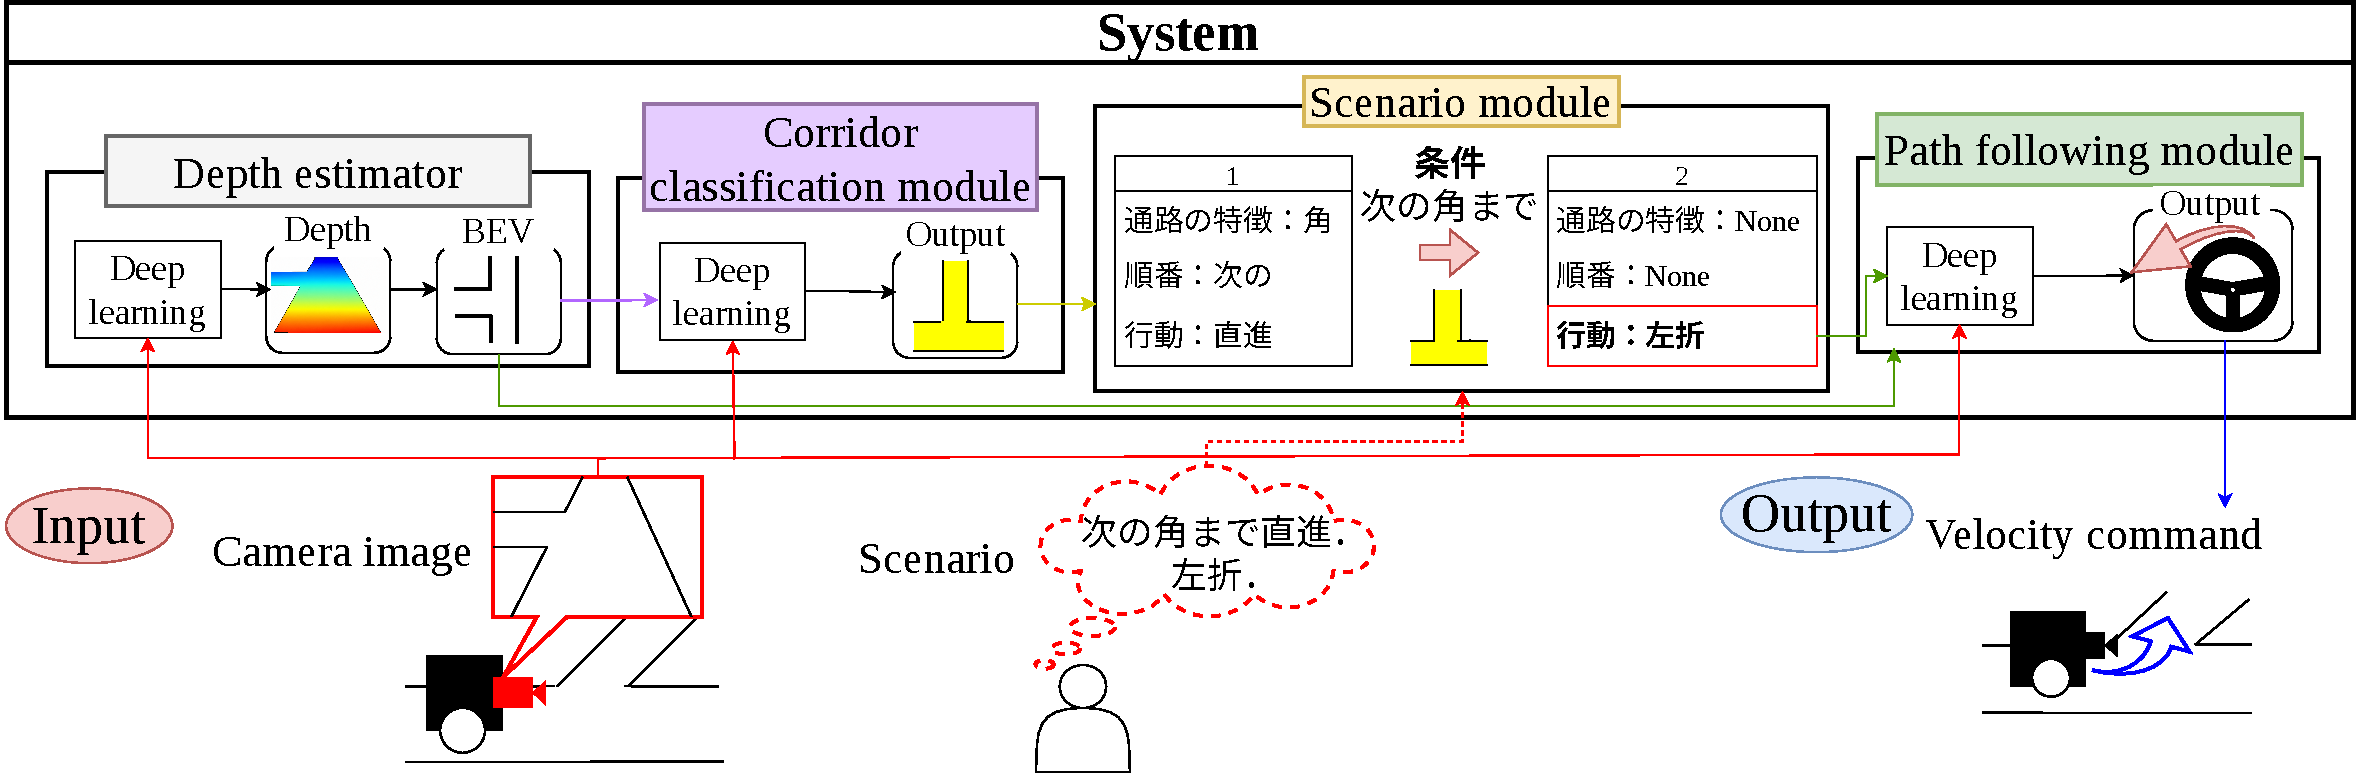
\includegraphics[width=\linewidth]{images/system.pdf}
  \caption{Scenario-driven navigation system}
  \label{fig:system}
\end{figure}

\section{ナビゲーションの流れ}
\label{sec:flow}

ナビゲーションの流れを以下に示す．
ロボットは，（a）で記述したシナリオを（b）で分解したのち，（c）から（e）を繰り返すことで，シナリオで指示された経路に沿って自律移動する．
\begin{enumerate}[label=（\alph*）,leftmargin=*,labelsep=0pt]
  \item 人間が，目的地までの道順を条件と行動の組として記述する．例えば，「次の角まで直進．左折．」というシナリオを作成する．
  \item シナリオモジュールがシナリオを分解し，条件と行動を抽出する．上記の例では，「次の角まで」を条件，「直進」を行動として取得する．
  \item シナリオモジュールが「直進」を目標方向として経路追従モジュールへ与え，経路追従モジュールはこの目標方向に沿ってロボットを走行させる．
  \item ロボットが角へ接近すると，通路分類モジュールが通路形状を「角」と分類する．シナリオモジュールは分類結果から「次の角まで」という条件が成立したと判定し，次の行動へ遷移する．
  \item シナリオモジュールが「左折」を新たな目標方向として経路追従モジュールへ与える．経路追従モジュールは新しい目標方向に従って角を左折する．
\end{enumerate}

\section{設計方針}
\label{sec:policy}

本研究では，ファインチューニングに用いていない環境においても，目的地まで移動可能かを調査する．
そのため，通路分類と経路追従には大規模データで事前学習された基盤モデルを用い，単一の環境で収集したデータによるファインチューニングで事前学習の表現が損なわれないようにする．
具体的には，基盤モデルの特徴抽出器を凍結し，主に新たに追加した部分を学習する．

単一の環境で収集したデータは，床や壁の色，照明などの外観が限られている．
このデータで特徴抽出器まで更新すると，モデルが学習環境の外観に依存した特徴を獲得し，外観の異なる環境で性能が低下するおそれがある．
特徴抽出器を凍結し，追加した小さな部分だけを学習すれば，事前学習で獲得された汎用的な表現をそのまま利用しつつ，本研究のタスクに必要な出力を得られると考える．
また，見た目に依存しにくい幾何的な情報として，単眼深度推定の結果を併用する．

\section{シナリオモジュール}
\label{sec:scenario_module}

シナリオモジュールは従来手法\cite{scenario_si2023}から変更していない．
シナリオの各文は1つの状態に対応し，各状態は「通路の特徴」「順番」「行動」の3要素で表される（\figref{fig:system}）．
例えば，「次の角まで直進．」は，通路の特徴を「角」，順番を「次の」，行動を「直進」とする状態となる．
通路の特徴と順番は状態の終了条件を表し，行動は目標方向を表す．
シナリオモジュールは，通路分類結果が終了条件を満たすと次の状態へと遷移し，新しい目標方向を経路追従モジュールへ送る．
目標方向は，直進，左折，右折の3通りである．

シナリオの文は形態素解析により単語に分割し，あらかじめ定めた語彙と照合して各要素を取り出す．
シナリオで用いる語彙を\tabref{tab:scenario_vocabulary}に示す．
通路の特徴には「左手に」「右手に」のように方向を付けることができ，「左手に通路が見えるまで直進．」は，左側に分岐が現れるまで直進することを表す．
順番は「3番目の三叉路まで」のように数で指定し，省略した場合は次に現れる通路を対象とする．

\begin{table}[tb]
  \centering
  \caption{Vocabulary of the scenario}
  \label{tab:scenario_vocabulary}
  \begin{tabular}{lp{0.7\linewidth}}
    \toprule
    要素 & 語彙 \\
    \midrule
    通路の特徴 & 一本道，三叉路，行き止まり，十字路，突き当り，曲がり角，角，通路，交差点 \\
    方向 & 前，前方，右，右手，左，左手，後ろ，後方 \\
    順番 & 〜つ目，〜番目，次 \\
    行動 & 直進，前進，右折，左折，向く，曲がる，停止 \\
    \bottomrule
  \end{tabular}
\end{table}

% TODO: 語彙は scenario_navigation/scripts/scenario_parser_jsk.py から取った．
%       「突き当り」と「行き止まり」の違いなど，条件判定の規則（cmd_dir_executor_detailed.cpp）を確認して書き足す．

\section{通路分類モジュール}
\label{sec:corridor_classifier}

\subsection{概要}

通路分類モジュールの構成を\figref{fig:corridor_classifier}に示す．
本モジュールは，直進方向，右分岐，左分岐の有無を推定し，その組合せから通路形状を出力する．
例えば，直進方向と右分岐が存在し，左分岐が存在しないと判定した場合，「三叉路右」という通路形状を出力する．
3方向の有無と通路形状の対応を\tabref{tab:passage_directions}に示す．
通路形状を直接分類するのではなく，3方向の有無を独立に推定することで，それぞれの出力が画像中の左，中央，右の領域の見え方と対応し，学習データの少ない通路形状でも各方向の判定を共有できる．

\begin{table}[tb]
  \centering
  \caption{Passage classes and the presence of each direction}
  \label{tab:passage_directions}
  \begin{tabular}{lccc}
    \toprule
    Passage class & Front & Left & Right \\
    \midrule
    straight\_road & \checkmark & & \\
    3\_way\_left   & \checkmark & \checkmark & \\
    3\_way\_right  & \checkmark & & \checkmark \\
    3\_way\_center & & \checkmark & \checkmark \\
    cross\_road    & \checkmark & \checkmark & \checkmark \\
    corner\_left   & & \checkmark & \\
    corner\_right  & & & \checkmark \\
    dead\_end      & & & \\
    \bottomrule
  \end{tabular}
\end{table}

% TODO: 表の対応はクラス名から整理したもの．corridor_classifier の実装と一致するか確認する．

\begin{figure}[tb]
  \centering
  \resizebox{\linewidth}{!}{% 通路分類モジュールの詳細図．paper.tex から \input して使う．
% 画像・BEV は未学習環境 m の実データおよび UniDepth の実出力．
% 各ブロックは隣のブロックからの間隔（\gap）で配置する．
\begin{tikzpicture}[
    font=\normalsize,
    blk/.style={draw, align=center, minimum height=8mm, minimum width=16mm,
                inner xsep=2pt},
    val/.style={draw, align=center, minimum height=6.5mm, minimum width=10mm},
    pic/.style={draw, inner sep=0pt},
    grp/.style={draw, dashed, gray},
    frz/.style={fill=cyan!12},
    lbl/.style={font=\small, inner sep=1.5pt},
    ar/.style={-{Latex[length=1.6mm]}, thin},
]
\def\gap{3mm}
% BEV 枝は UniDepth から 128-D までを等間隔にする（上段の幅から決めた値）．
\def\botgap{7.4mm}
% 各行の高さ
\coordinate (top) at (0,0);
\coordinate (mid) at (0,-1.8);
\coordinate (bot) at (0,-3.6);

% ---- 入力 ----------------------------------------------------------------
\node[pic] (rgb) at (0,-1.7) {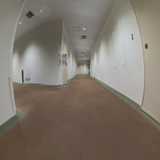
\includegraphics[width=13mm]{images/cc_rgb.png}};
\node[lbl, below=0.5mm of rgb] {RGB image};
\coordinate (rsplit) at ([xshift=2.5mm]rgb.east);

% ---- RGB 枝 --------------------------------------------------------------
\node[blk, anchor=west] (res) at ([xshift=\gap]rsplit |- top) {Resize\\$224\times224$};
\node[blk, frz, right=\gap of res] (dno) {\DINOvTwo\ ViT\text{-}S/14\\\small \frozen};
\node[blk, right=\gap of dno] (rdo) {Spatial readout\\\small CLS $+$ 3 regional means};
\node[val, right=\gap of rdo] (f15) {$1536$\text{-}D};
\node[pic] (b2) at (rdo |- 0,-1.4) {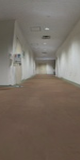
\includegraphics[width=6mm]{images/cc_band2.png}};
\node[pic] (b1) at ([xshift=-7mm]b2) {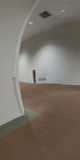
\includegraphics[width=6mm]{images/cc_band1.png}};
\node[pic] (b3) at ([xshift=7mm]b2) {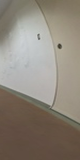
\includegraphics[width=6mm]{images/cc_band3.png}};
\node[lbl, below=0.5mm of b2] {left \,\textbar\, center \,\textbar\, right};

% ---- BEV 枝 --------------------------------------------------------------
\node[blk] (udp) at (res |- bot) {\UniDepth};
\node[pic, right=\botgap of udp] (dep) {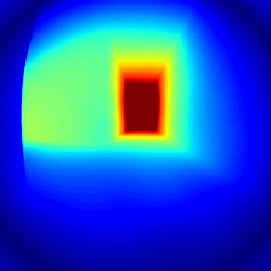
\includegraphics[width=11mm]{images/pf_depth_cmap.png}};
\node[pic, right=\botgap of dep] (bev) {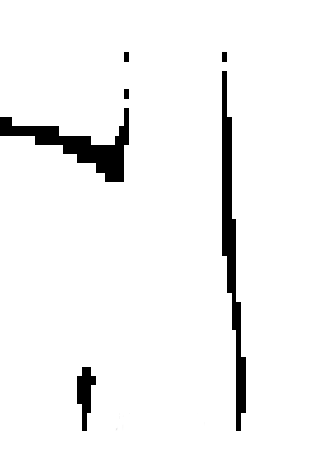
\includegraphics[height=15mm]{images/cc_bev_inner.png}};
\draw (bev.south west) rectangle (bev.north east);
\node[lbl, below=0.5mm of bev] {BEV $50\times70$};
\node[blk, right=\botgap of bev] (cnn) {BEV CNN\\\small $4\times4$ pooling};

% ---- 分類ヘッド ----------------------------------------------------------
% 1536-D と 128-D は Feature fusion の真上と真下に置き，縦の矢印で結ぶ．
\node[blk] (fus) at (f15 |- mid) {Feature fusion\\\small $256$\text{-}D};
\node[val] (f12) at (f15 |- bot) {$128$\text{-}D};
\node[blk, right=\gap of fus] (gru) {GRU\\\small 3 frames, stride 4};
\node[blk, right=\gap of gru] (lin) {Linear $+$\\sigmoid};
\node[val, minimum width=13mm, right=4mm of lin] (pr) {$p(\mathrm{right})$};
\node[val, minimum width=13mm, above=2.5mm of pr] (pf) {$p(\mathrm{front})$};
\node[val, minimum width=13mm, below=2.5mm of pr] (pl) {$p(\mathrm{left})$};

% ---- 結線 ----------------------------------------------------------------
\draw[thin] (rgb.east) -- (rsplit);
\draw[ar] (rsplit) |- (res.west);
\draw[ar] (rsplit) |- (udp.west);
\draw[ar] (res) -- (dno);
\draw[ar] (dno) -- (rdo);
\draw[ar] (rdo) -- (f15);
\draw[ar] (udp) -- (dep);
\draw[ar] (dep) -- (bev);
\draw[ar] (bev) -- (cnn);
\draw[ar] (cnn) -- (f12);
\draw[ar] (f15) -- (fus);
\draw[ar] (f12) -- (fus);
\draw[ar] (fus) -- (gru);
\draw[ar] (gru) -- (lin);
\draw[ar] (lin.east) -- (pf.west);
\draw[ar] (lin.east) -- (pl.west);
\draw[ar] (lin.east) -- (pr.west);

\end{tikzpicture}
}
  \caption{Corridor-classification module}
  \label{fig:corridor_classifier}
\end{figure}

\subsection{RGB画像の特徴}

視覚特徴の抽出には\DINOvTwo を用いる．\DINOvTwo のパラメータは学習時にすべて凍結し，大規模データによる事前学習で獲得された視覚表現を保持する．
単一の棟で収集したデータに対して特徴抽出器まで更新すると，学習環境の外観に過度に適合するおそれがあるためである．

モデルにはViT-S/14を用い，入力画像は$224\times224$にリサイズする．
最終層のCLSトークンに加え，パッチトークンを画像の左，中央，右の3つの縦長の領域に分けて領域ごとに平均する．
CLSトークンは画像全体の特徴を表すが，分岐がどちら側にあるかという位置の情報は失われやすい．
領域ごとの平均を併用することで，左右の分岐の有無を判定するための位置の情報を保持する．
CLSトークンと3つの領域の平均はそれぞれ384次元であり，これらを結合した1536次元のベクトルをRGB画像の特徴とする．

\subsection{鳥瞰の占有格子}

また，見た目に依存しにくい情報として，\UniDepth により推定した深度から床面と天井を除いた壁面および障害物の点群を求め，水平面へ投影した鳥瞰（BEV: Bird's-Eye View）の占有格子を併用する．
具体的には，推定深度から求めた点群のうち，高さ$\SI{0.05}{m}$から$\SI{1.6}{m}$の点を壁面および障害物とする．
これらの点を，前方$\SI{0.1}{m}$から$\SI{5.1}{m}$，左右$\pm\SI{3.5}{m}$の範囲で，一辺$\SI{0.1}{m}$の格子に投影し，$50\times70$の占有格子を作成する．
各格子には，点が存在するかどうかを2値で与える．
点の数をそのまま用いると，カメラからの距離や壁面の材質によって値が変わるためである．

占有格子は小さなCNNで処理し，出力を$4\times4$の領域ごとに平均して128次元の特徴とする．
格子全体を1つの値に平均すると，通路の開口部がどこにあるかという情報が失われるため，領域ごとに平均して位置の情報を残す．

\subsection{時系列の統合と出力}

そして，\DINOvTwo の特徴とBEVの特徴を結合し，GRU\cite{gru}により時系列情報を考慮して通路形状を分類する．
結合した特徴は全結合層で256次元に変換し，隠れ状態256次元の1層のGRUへ入力する．
GRUには，$0.25$\,s間隔の観測から4フレームおきに取り出した3フレームを与える．
GRUの出力は全結合層とシグモイド関数により，直進方向，左分岐，右分岐それぞれの存在確率に変換する．
各確率は閾値$0.5$で2値化し，\tabref{tab:passage_directions}に従って通路形状を求める．

学習では，3方向それぞれの有無に対する2値交差エントロピーを損失とする．
最適化にはAdamW\cite{adamw}を用い，追加した部分の学習率を$1\times10^{-3}$，重み減衰を$1\times10^{-4}$とし，学習率はコサインスケジュールで減衰させる．
% TODO: 要確認．値は corridor_classifier/config/model.yaml，training.yaml の現在の設定から取った．
%       SI原稿の実験で用いた重み（weights/production/bevwall_pool4.pth）を学習したときのエポック数（10か7か）とバッチサイズを確認する．

実行時は$4$\,Hzで推論する．
1フレームだけの誤分類で条件が成立しないよう，同じ分類結果が3フレーム連続したときに出力を切り替える．
また，学習データには旋回中の画像の通路形状を含めていないため，ロボットが旋回している間は推論を行わず，旋回中であることを出力する．
データセットの作成方法は\secref{sec:dataset}で述べる．

\section{経路追従モジュール}
\label{sec:path_following}

\subsection{目標方向による条件付け}

経路追従モジュールの構成を\figref{fig:path_following}に示す．
基本方策には，複数環境の走行データで事前学習された視覚ナビゲーション基盤モデル\NoMaD を用い，ゴール画像の代わりにシナリオモジュールから与えられる目標方向を入力する．
ゴール画像は常にマスクする．
\NoMaD は，現在と過去3フレームの計4フレームの画像（$96\times96$）をEfficientNet-B0\cite{efficientnet}で符号化し，Transformerで統合して256次元の条件ベクトルを得る．
この条件ベクトルを条件として，拡散モデルが将来8点のwaypoint列を生成する．

目標方向は埋め込みベクトルに変換し，\NoMaD の視覚エンコーダがRGB画像から得る条件ベクトルへ加算する．
目標方向は直進，左折，右折の3通りのone-hotベクトルで表し，3層の多層パーセプトロンで条件ベクトルと同じ次元の埋め込みに変換する．
条件ベクトルを置き換えるのではなく加算とするのは，事前学習で獲得された観測の表現をできるだけ保ったまま，目標方向の情報を付加するためである．

\begin{figure}[tb]
  \centering
  \resizebox{\linewidth}{!}{% 経路追従モジュールの詳細図．paper.tex から \input して使う．
% 観測画像と深度マップは未学習環境 m の実データおよび UniDepth の実出力．
% CARE の補正を表す top-down の模式図は例示．
\begin{tikzpicture}[
    font=\normalsize,
    x=0.85cm,
    blk/.style={draw, align=center, minimum height=8mm, minimum width=16mm,
                inner xsep=2pt},
    val/.style={draw, align=center, minimum height=6.5mm, minimum width=9mm},
    pic/.style={draw, inner sep=0pt},
    grp/.style={draw, dashed, gray},
    frz/.style={fill=cyan!12},
    lbl/.style={font=\small, inner sep=1.5pt},
    ar/.style={-{Latex[length=1.6mm]}, thin},
]
% ---- 観測 ----------------------------------------------------------------
\node[pic] (o3) at (0,0) {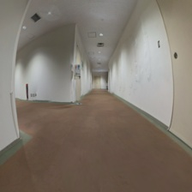
\includegraphics[width=15mm]{images/pf_obs3.png}};
\node[pic] (o2) at (-0.1,0.1) {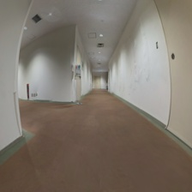
\includegraphics[width=15mm]{images/pf_obs2.png}};
\node[pic] (o1) at (-0.2,0.2) {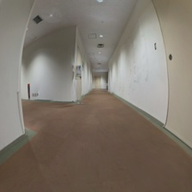
\includegraphics[width=15mm]{images/pf_obs1.png}};
\node[lbl, below=0.5mm of o3, align=center] {RGB images\\$4$ frames};

% ---- NoMaD 本体 ----------------------------------------------------------
\node[blk, frz] (enc) at (3.9,0) {Image encoder\\\small EfficientNet\text{-}B0, \frozen};
\node[blk, frz] (trn) at (7.8,0) {Transformer\\\small \frozen};
\node[circle, draw, inner sep=1.2pt] (sum) at (10.2,0) {$+$};
\node[blk, minimum width=21mm] (dif) at (13.5,0)
      {Diffusion policy\\\small $8$ waypoints};

% ---- 目標方向（本研究で追加）---------------------------------------------
% 直進・左折・右折のアイコン．この例では左折を与えているため，左折を強調する．
\def\diricon#1#2{\tikz[baseline=0, line width=1pt, rounded corners=1.1mm]
    \draw[-{Latex[length=1.8mm, width=2.1mm]}, #1] #2;}
\def\diricons{\diricon{}{(0,0) -- (0,4.2mm)}\quad
    \diricon{red, line width=1.8pt}{(0,0) |- (-2.9mm,3mm)}\quad
    \diricon{}{(0,0) |- (2.9mm,3mm)}}
\node[blk, fill=black!8, minimum width=21mm] (cmd) at (3.6,-1.7) {Target direction\\[0.5mm]\diricons};
\node[blk, fill=black!8] (den) at (7.8,-1.7) {Direction encoder\\\small 3\text{-}layer MLP};

% ---- 深度・障害物 --------------------------------------------------------
\node[blk, minimum width=18mm] (udp) at (3.6,-3.7) {\UniDepth};
\node[pic] (dep) at (6.6,-3.7) {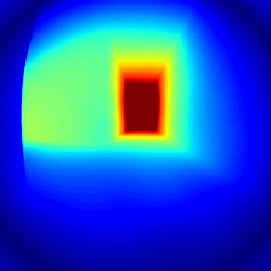
\includegraphics[width=13mm]{images/pf_depth_cmap.png}};
\node[pic] (bev) at (9.6,-3.7) {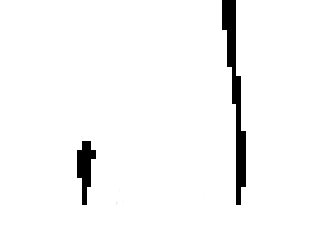
\includegraphics[height=13mm]{images/pf_bev_cc_noarrow.png}};
\draw (bev.south west) rectangle (bev.north east);
\node[lbl, below=0.5mm of bev] {BEV};

% ---- CARE ----------------------------------------------------------------
\node[blk] (care) at (13.5,-3.7) {\CARE};
\node[val] (vw)  at (17.95,-3.7) {$(v,\omega)$};

% ---- CARE による補正の模式図（例示）--------------------------------------
% 背景は BEV と同じ画像（幅 1.9 の座標系に合わせて軌道を重ねる）．
% scale で画像幅 2.4cm に合わせて座標系ごと拡大する．
\begin{scope}[shift={(16.75,-2.4)}, x=1cm, y=1cm, scale=2.4/1.9]
  \node[anchor=south west, inner sep=0pt] at (0,0)
        {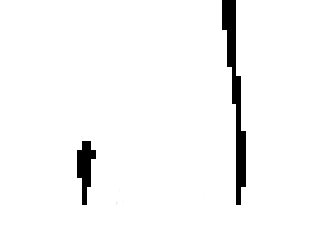
\includegraphics[width=2.4cm]{images/pf_bev_cc_noarrow.png}};
  \draw (0,0) rectangle (1.9,1.365);
  \draw[densely dashed, gray, thick] (0.96,0.17)
        .. controls (0.96,0.45) and (0.8,0.62) .. (0.3,0.68)
        node[lbl, below, inner sep=1.5pt] {$p_k$};
  \draw[thick] (0.96,0.17)
        .. controls (0.96,0.7) and (0.8,0.95) .. (0.2,1.0)
        node[lbl, pos=0.8, above, inner sep=1.5pt] {$p'_k$};
  \node[lbl, anchor=north] (toplab) at (0.95,0) {example};
\end{scope}
\coordinate (topsw) at (16.75,-2.4);

% ---- 結線 ----------------------------------------------------------------
\draw[ar] (o3) -- (enc);
\draw[ar] (enc) -- (trn);
\draw[ar] (trn) -- (sum);
\draw[ar] (sum) -- (dif);
\draw[ar] (cmd) -- (den);
\draw[ar] (den.east) -| (sum.south);
\draw[ar] (o1.west) -- ++(-0.35,0) |- (udp.west);
\draw[ar] (udp) -- (dep);
\draw[ar] (dep) -- (bev);
\draw[ar] (dif.south -| care.north) -- (care.north);
\draw[ar] (bev) -- (care);
\draw[ar] (care) -- (vw);
\draw[black!60, densely dashed, thick] (care.north east) -- (topsw);


% ---- 枠 ------------------------------------------------------------------
\begin{scope}[on background layer]
  \node[grp, fit=(enc)(dif)(cmd)(den), inner sep=3mm] (gn) {};
\end{scope}
\node[lbl, anchor=north west, fill=white, inner xsep=2pt]
      at ([xshift=2mm,yshift=0.2mm]gn.north west) {Direction\text{-}conditioned \NoMaD};
\end{tikzpicture}
}
  \caption{Path-following module}
  \label{fig:path_following}
\end{figure}

\subsection{学習}

学習は2段階で行い，視覚エンコーダは両段階を通じて凍結する．
目標方向の埋め込みは学習初期には十分に形成されていないため，第1段階では拡散モデルも凍結し，目標方向の埋め込みのみを学習する．
これにより，事前学習済みの拡散モデルを保持したまま，目標方向の埋め込みを学習する．
第2段階では拡散モデルの凍結を解き，小さい学習率で適合させる．

第1段階では，目標方向の埋め込みの学習率を$5\times10^{-4}$とし，20エポック学習する．
第2段階では，拡散モデルの学習率を$2\times10^{-6}$，目標方向の埋め込みの学習率を$5\times10^{-5}$とし，12エポック学習する．
いずれの段階も，バッチサイズを64とし，学習率はウォームアップの後にコサインスケジュールで減衰させる．
% TODO: 要確認．値は vnm_ros/config/experiments/nomad_yawfix_staged_stage1，stage2 の nomad.yaml から取った．
%       SI原稿の実験でこの設定の重みを用いたか確認する．

目標方向のラベルは直進に偏るため（\tabref{tab:dataset}），損失には各方向の出現頻度に応じた重みを与える．
目標方向$c$のサンプル数を$N_c$とすると，その重み$w_c$を
\begin{equation}
  w_c \propto N_c^{-1/2}
  \label{eq:loss_weight}
\end{equation}
とし，全サンプルにわたる重みの平均が1となるように正規化する．
出現頻度の逆数をそのまま用いると，サンプル数の少ない左折と右折の重みが大きくなりすぎるため，平方根をとって偏りを緩和する．

\subsection{推論と衝突回避}

推論時は，拡散モデルから複数のwaypoint列を生成してその平均を基準の軌道とし，障害物からの反発力に基づく衝突回避手法\CARE\cite{care}により補正する．
生成するwaypoint列は8本とし，拡散モデルの反復回数は10回とする．
\CARE には，\UniDepth が推定した深度から求めた前方近傍の点群を障害物として与える．
これにより，幾何情報に基づく安全性を付加することを狙う．
補正後の軌道上の1点を目標として選び，その方位から並進速度と角速度を算出する．

目標点のロボット座標系における位置を$(x, y)$，制御周期を$\Delta t$とすると，並進速度$v$と角速度$\omega$は次式で求める．
\begin{equation}
  v = \frac{x}{\Delta t}, \qquad
  \omega = \frac{1}{\Delta t}\arctan\frac{y}{x}
  \label{eq:control}
\end{equation}
これはViNTおよび\NoMaD の参照実装と同じ制御則である．
求めた速度は，並進速度$\SI{0.2}{m/s}$，角速度$\SI{0.3}{rad/s}$を上限として制限する．
% TODO: 要確認．制御周期（model_rate 3 Hz），速度の上限，目標点の番号は
%       vnm_ros/config/experiments/nomad_yawfix_staged_stage2/runtime.yaml，nomad.yaml，config/care.yaml から取った．
%       目標点の番号が nomad.yaml（waypoint_index: 2）と care.yaml（waypoint_index: 4）で異なるので，実験時の値を確認する．

%!TEX root = ../../thesis.tex
\chapter{実験}
\label{chap:experiment}

本章では，構築したシステムが，データを収集していない環境でもシナリオに従って目的地まで移動できるかを，シミュレータ上で検証する．

\section{実験環境}
\label{sec:experiment_env}

実験環境として，千葉工業大学2号館3階の高層棟と低層棟を3次元再構成した2つのシミュレータ環境を用いる．
それぞれの環境を\figref{fig:sim_env}に示す．
高層棟を，データを収集した学習環境とし，低層棟を学習に用いない未学習環境とする．
両者は，床や壁の色，エレベーターの有無などの外観が異なる．
シナリオは高層棟7例，低層棟6例を用意する．各環境のシナリオと経路を\figref{fig:scenario}，\figref{fig:scenario_unseen}に，シナリオの文を\tabref{tab:scenarios}に示す．
シナリオには，直進のみのもの，左折と右折を含むもの，「左手に通路が見えるまで」のように方向を指定した条件を含むものがある．

\begin{table}[tb]
  \centering
  \caption{Scenarios used in the experiment}
  \label{tab:scenarios}
  \small
  \begin{tabular}{clp{0.72\linewidth}}
    \toprule
    No. & 環境 & シナリオ \\
    \midrule
    01 & 高層棟 & 3番目の三叉路まで直進．停止． \\
    02 & 高層棟 & 2番目の三叉路まで直進．左折．突き当りまで直進．停止． \\
    03 & 高層棟 & 突き当りまで直進．左折．左手に通路が見えるまで直進．左折．右手に通路が見えるまで直進．右折．左手に曲がり角が見えるまで直進．左折．突き当りまで直進．停止． \\
    04 & 高層棟 & 突き当りまで直進．左折．左手に通路が見えるまで直進．左折．右手に通路が見えるまで直進．右折．左手に曲がり角が見えるまで直進．左折．突き当りまで直進．右折．突き当りまで直進．停止． \\
    05 & 高層棟 & 右手に曲がり角が見えるまで直進．右折．突き当りまで直進．左折．突き当りまで直進．停止． \\
    06 & 高層棟 & 突き当りまで直進．右折．左手に通路が見えるまで直進．左折．三叉路まで直進．停止． \\
    07 & 高層棟 & 左を向く．突き当りまで直進．右折．右手に曲がり角が見えるまで直進．右折．突き当りまで直進．停止． \\
    08 & 低層棟 & 突き当りまで直進．停止． \\
    09 & 低層棟 & 左手に曲がり角が見えるまで直進．左折．突き当りまで直進．右折．突き当りまで直進．停止． \\
    10 & 低層棟 & 突き当りまで直進．左折．突き当りまで直進．停止． \\
    11 & 低層棟 & 突き当りまで直進．停止． \\
    12 & 低層棟 & 次の角まで直進．右折．突き当りまで直進．右折．突き当りまで直進．停止． \\
    13 & 低層棟 & 次の角まで直進．右折．突き当りまで直進．停止． \\
    \bottomrule
  \end{tabular}
\end{table}

% TODO: 要確認．シナリオの文は scenario_navigation/config/Scenarios/scenario{01..07,16,17,27,31,36,37}.txt から取った
%       （図のファイル名 Scenario_16.pdf などとの対応で，No.08〜13 に振り直している）．

シミュレータにはGazeboを用い，ロボットの前方に取り付けた1台のカメラの画像を各モジュールへ入力する．

% TODO: ロボットのモデル，カメラの解像度と画角，学習と推論に用いた計算機を書く．

\begin{figure}[tb]
  \centering
  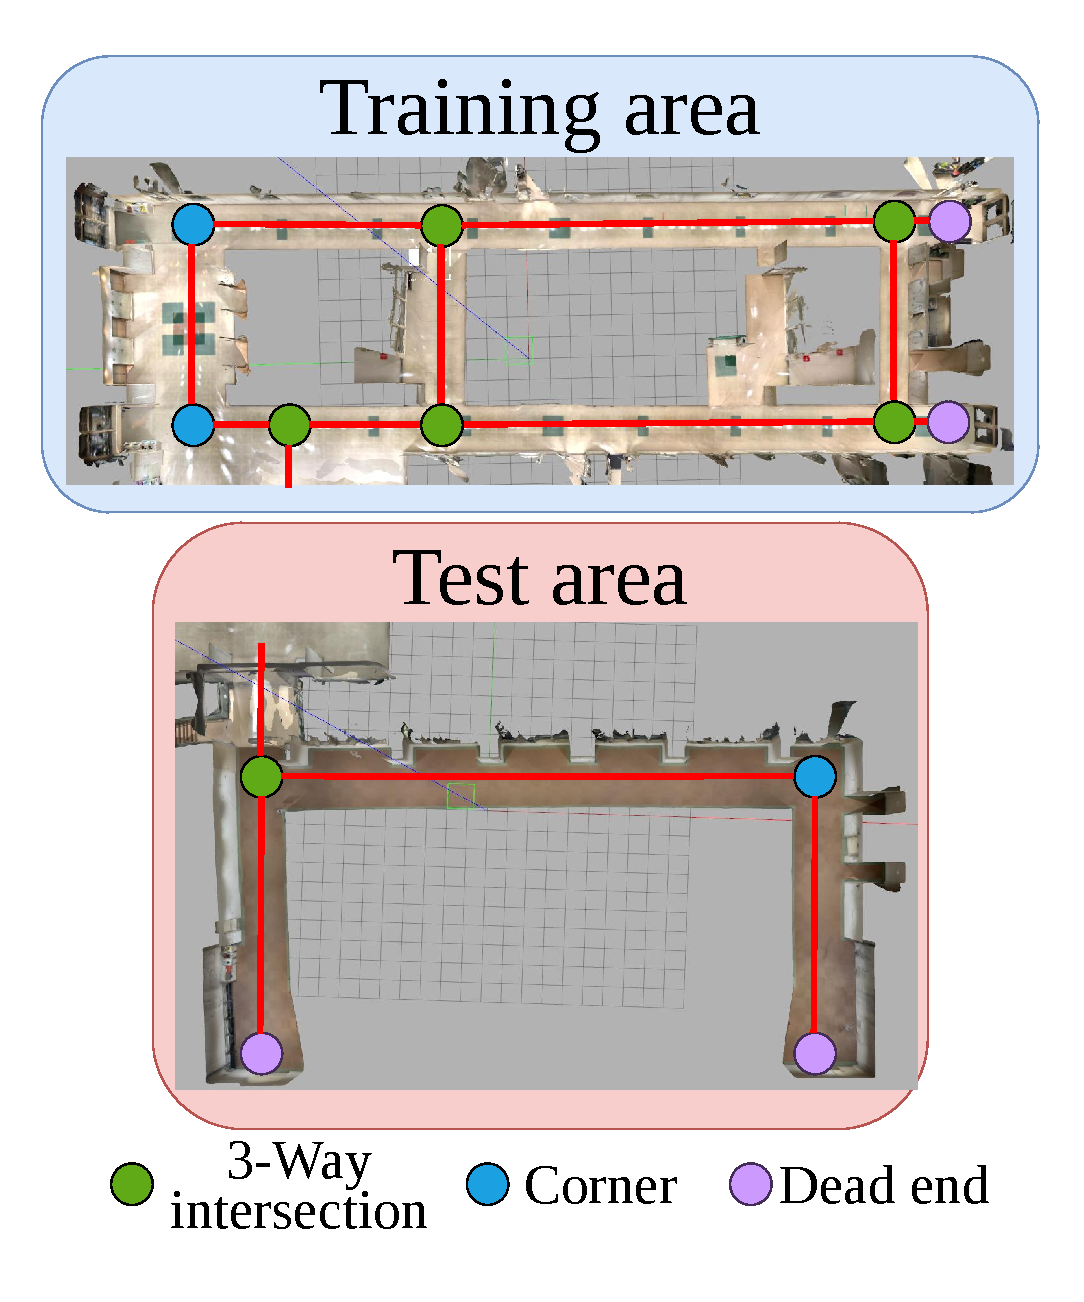
\includegraphics[width=0.86\linewidth]{images/enviroment.pdf}
  \caption{Simulator environments}
  \label{fig:sim_env}
\end{figure}

\section{データセット}
\label{sec:dataset}

データセットは，学習環境である高層棟でのみ作成する．
ROS navigationパッケージにより経由点列に沿ってロボットを走行させ，走行中のカメラ画像，自己位置および目標方向を$0.25$\,s間隔で記録する．
経由点にはあらかじめ通路形状と目標方向を設定し，記録時に各カメラ画像へ対応するラベルを自動的に付与する．
これにより，手動でラベルを付与することなく，データセットを構築できる．
高層棟を約$\SI{395}{m}$走行し，計$6069$サンプルを得た．
内訳を\tabref{tab:dataset}に示す．

通路分類モジュールの入力は$224\times224$に，経路追従モジュールの入力は$96\times96$にリサイズする．
経路追従の教師は，記録した自己位置から，各時刻のロボット座標系における$8$点のwaypoint列として算出する．

通路分類のラベルは，経由点に設定した通路形状を，次の経由点に到達するまでの画像に付与する．
ただし，旋回中の画像は通路形状が定まらないため，ロボットの角速度から旋回中と判定した区間を通路形状の学習から除く．
目標方向のラベルは，直進が全体の約7割を占め，左折と右折はそれぞれ約1.5割である（\tabref{tab:dataset}）．
通路形状も一本道が約半数を占め，行き止まりは48サンプルと少ない．

% TODO: 要確認．ラベル付けの規則（旋回区間の扱い）は corridor_classifier/config/dataset.yaml の turn_detection から推測したもの．

\begin{table}[tb]
  \centering
  \caption{Training dataset collected in the high-rise wing}
  \label{tab:dataset}
  \begin{tabular}{lr@{\qquad}lr}
    \toprule
    Passage class & Samples & Target direction & Samples \\
    \midrule
    straight\_road & 3140 & straight & 4269 \\
    3\_way\_left   &  738 & left     &  908 \\
    3\_way\_right  &  727 & right    &  892 \\
    3\_way\_center &  620 &          &      \\
    corner\_right  &  399 &          &      \\
    corner\_left   &  397 &          &      \\
    dead\_end      &   48 &          &      \\
    \midrule
    Total & 6069 & Total & 6069 \\
    \bottomrule
  \end{tabular}
\end{table}

\section{実験方法}
\label{sec:experiment_method}

実験は以下の手順で行う．
通路分類モデルと経路追従モデルは，高層棟のデータで1度だけ学習し，両方の環境で同じモデルを用いる．
\begin{enumerate}[label=\arabic*)]
  \item ROS navigationパッケージでロボットを走行させ，データを収集する．
  \item 収集したデータセットを用いて，通路分類モデルと経路追従モデルをファインチューニングする．
  \item シナリオの開始地点にロボットを配置する．
  \item シナリオを入力し，自律移動を開始する．
  \item 目的地へ到達するかを確認する．
\end{enumerate}

% TODO: 各シナリオの試行回数，成功の判定基準，記録する項目を書く．

\begin{figure}[p]
  \centering
  \begin{subfigure}[b]{0.32\linewidth}
    \centering
    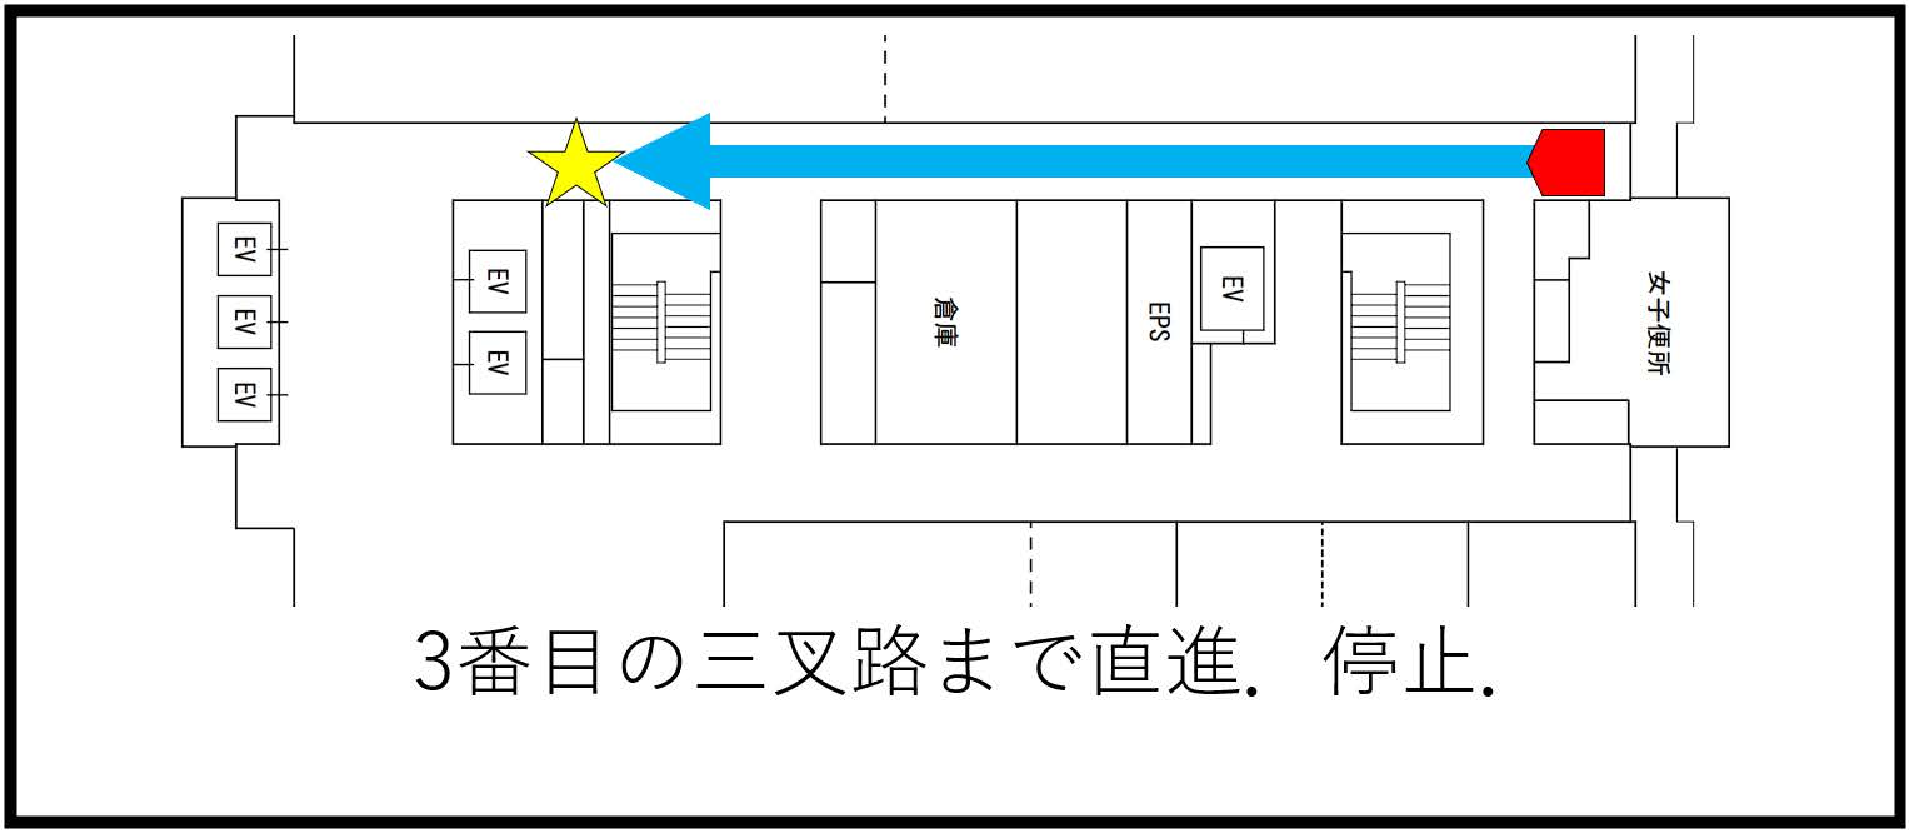
\includegraphics[width=\linewidth]{images/Scenario_01.pdf}
    \caption{Scenario 01}
  \end{subfigure}\hfill
  \begin{subfigure}[b]{0.32\linewidth}
    \centering
    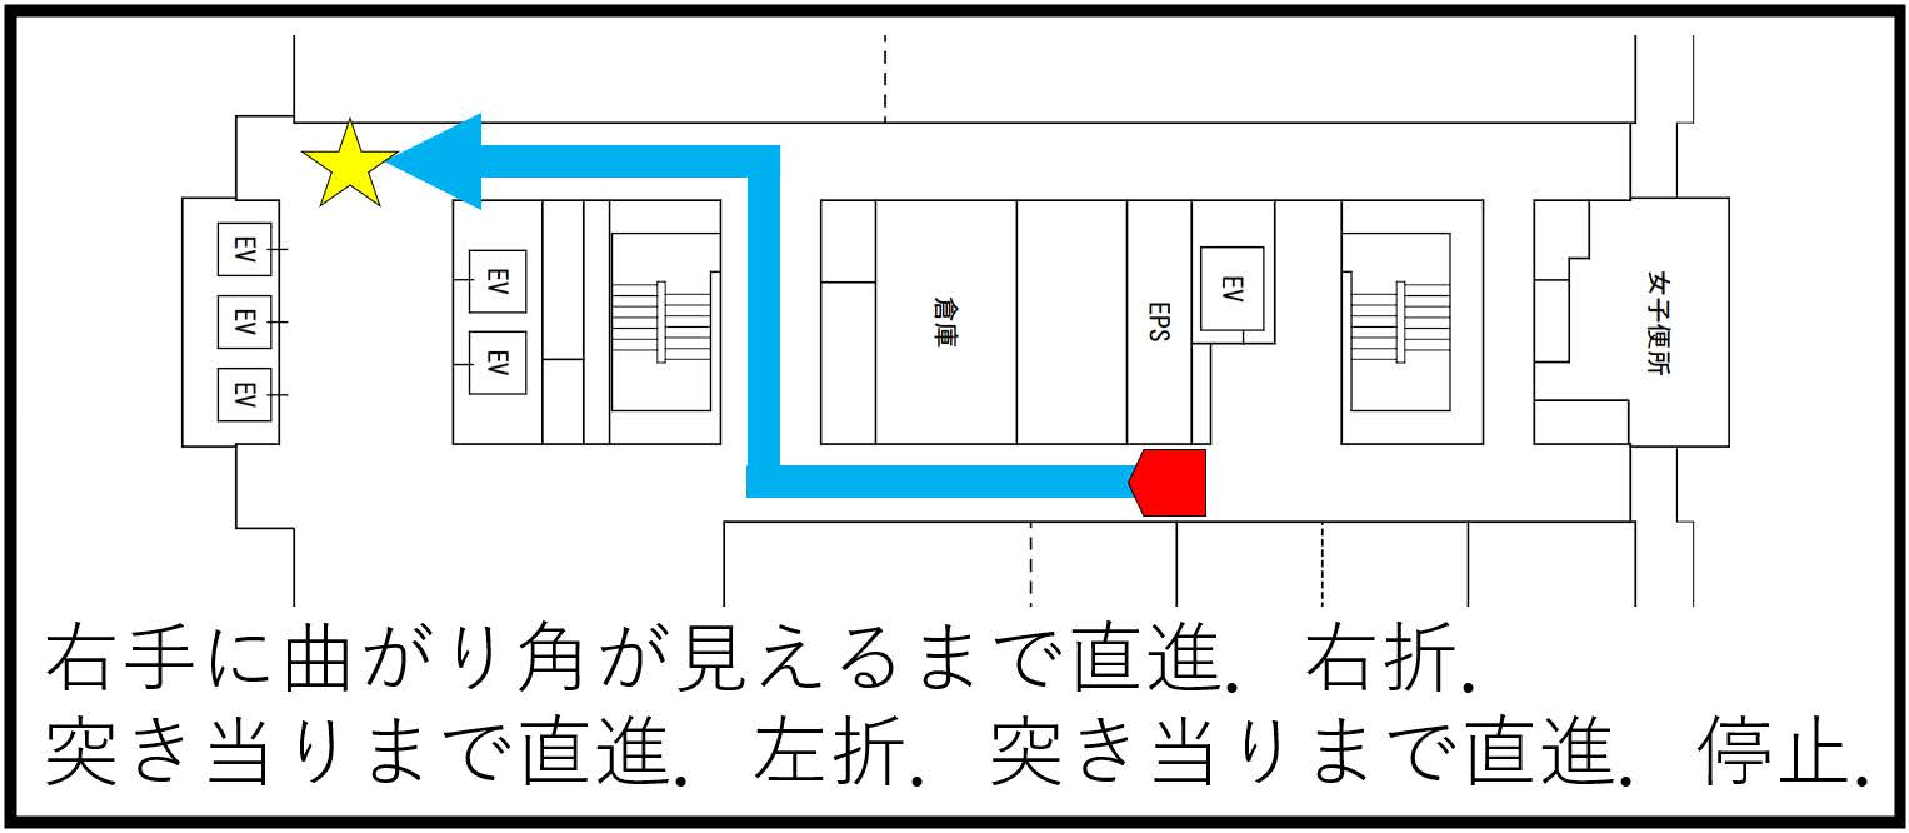
\includegraphics[width=\linewidth]{images/Scenario_02.pdf}
    \caption{Scenario 02}
  \end{subfigure}\hfill
  \begin{subfigure}[b]{0.32\linewidth}
    \centering
    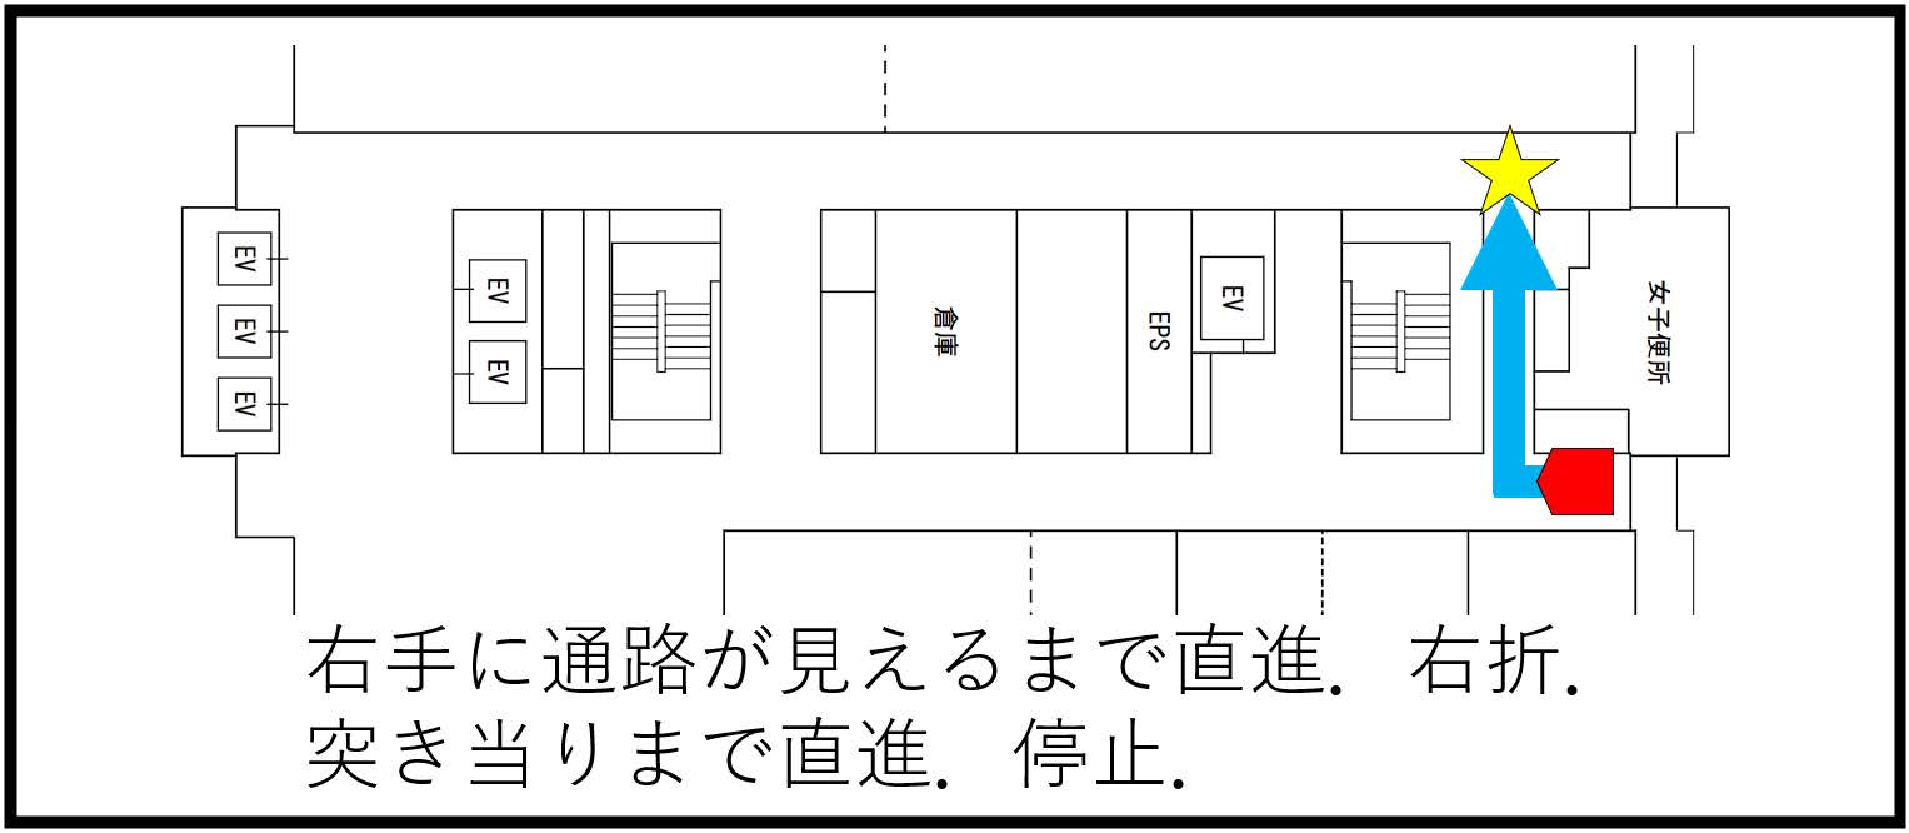
\includegraphics[width=\linewidth]{images/Scenario_03.pdf}
    \caption{Scenario 03}
  \end{subfigure}

  \vspace{0.5\baselineskip}

  \begin{subfigure}[b]{0.32\linewidth}
    \centering
    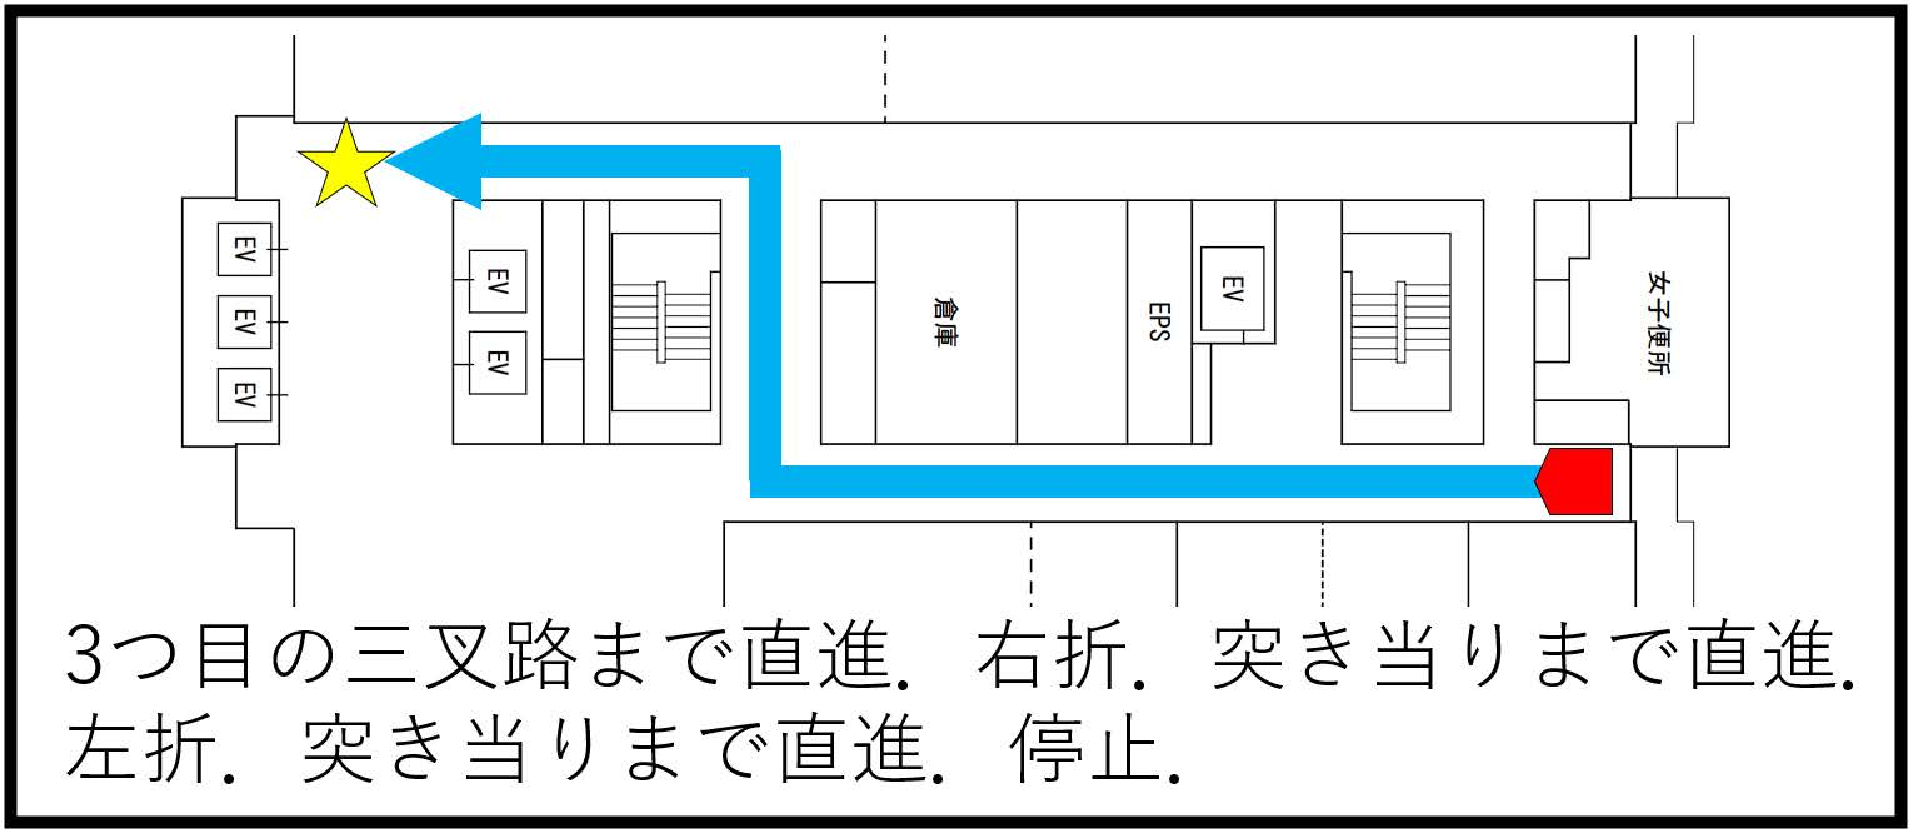
\includegraphics[width=\linewidth]{images/Scenario_04.pdf}
    \caption{Scenario 04}
  \end{subfigure}\hfill
  \begin{subfigure}[b]{0.32\linewidth}
    \centering
    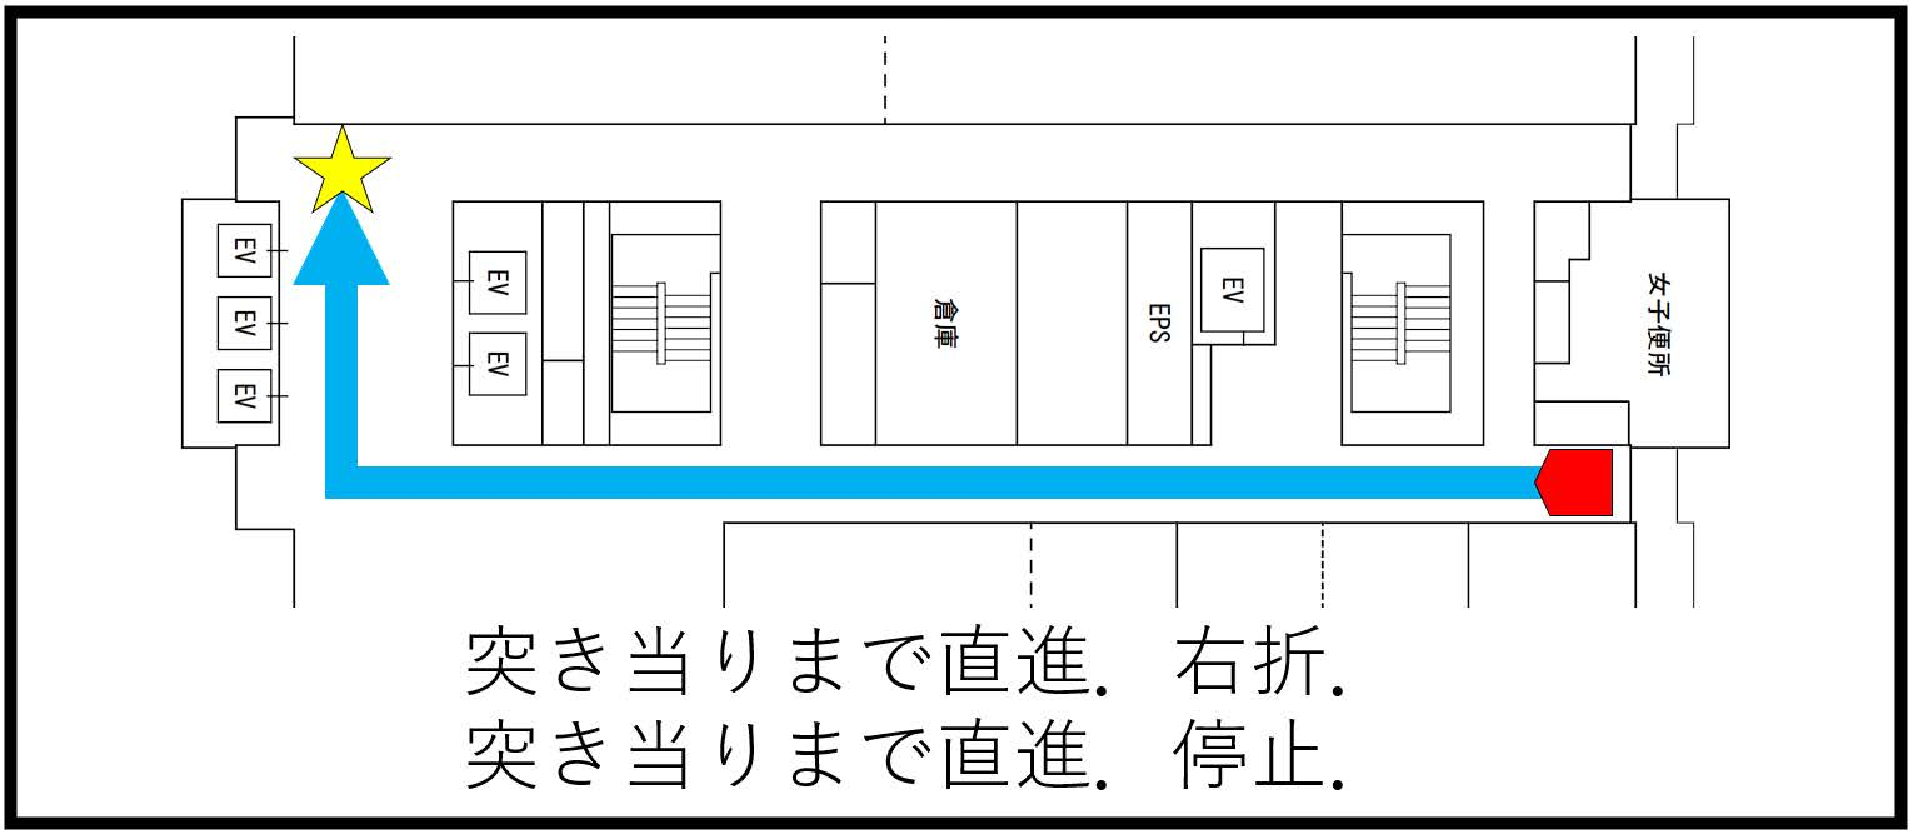
\includegraphics[width=\linewidth]{images/Scenario_05.pdf}
    \caption{Scenario 05}
  \end{subfigure}\hfill
  \begin{subfigure}[b]{0.32\linewidth}
    \centering
    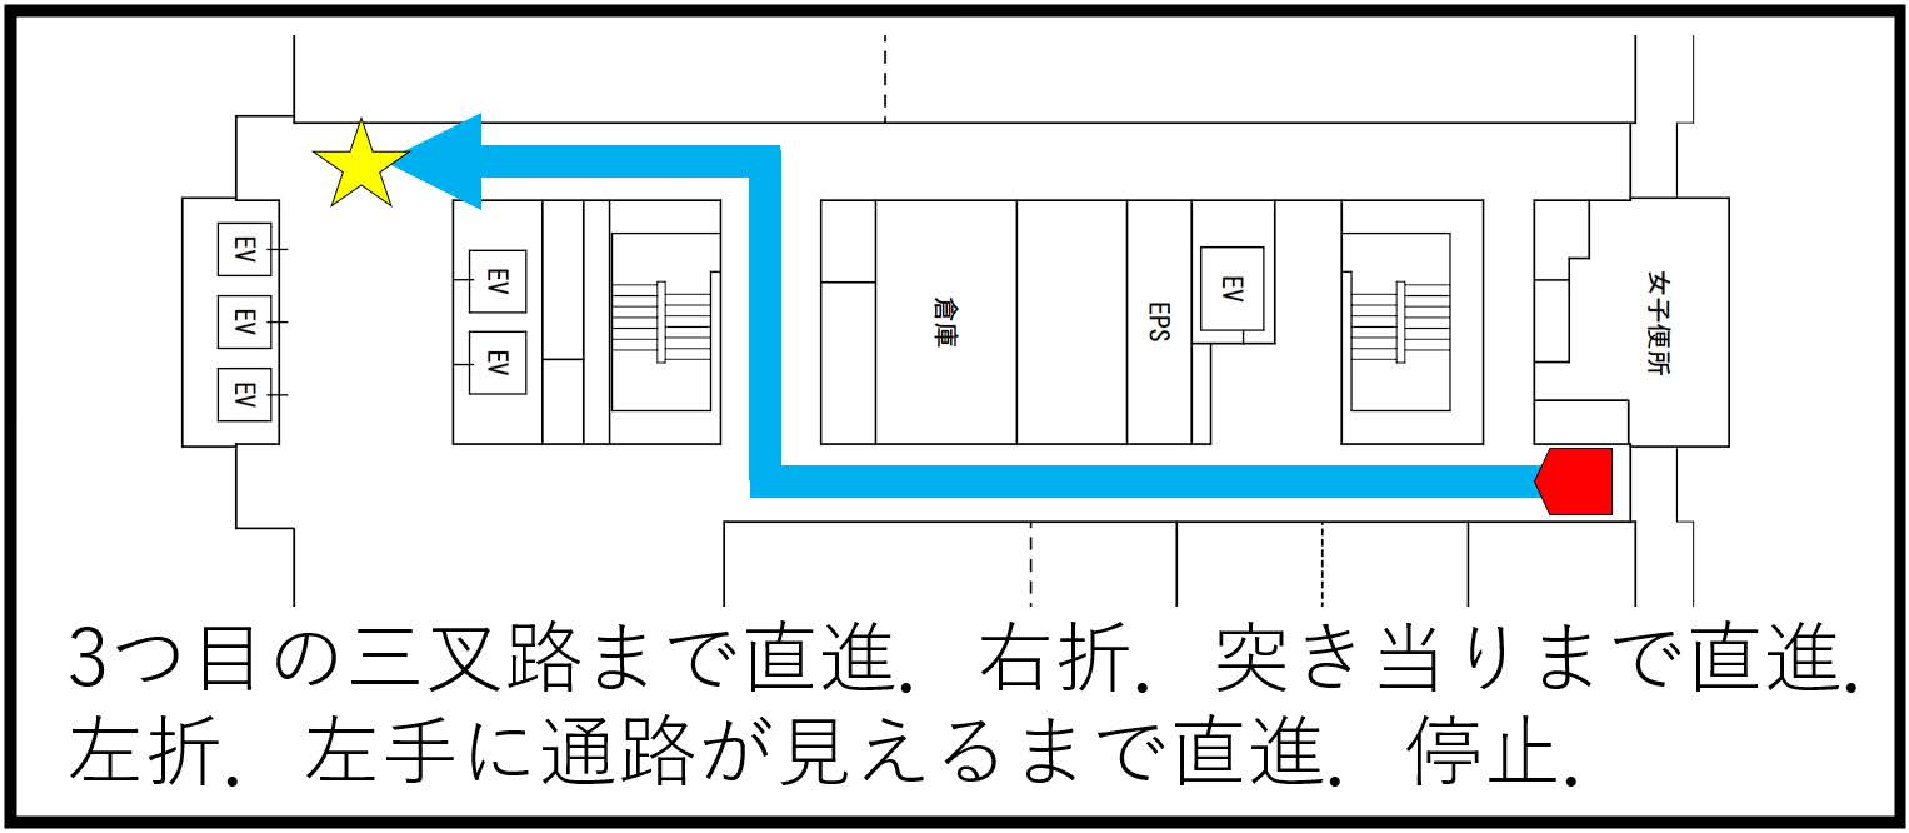
\includegraphics[width=\linewidth]{images/Scenario_06.pdf}
    \caption{Scenario 06}
  \end{subfigure}

  \vspace{0.5\baselineskip}

  \begin{subfigure}[b]{0.32\linewidth}
    \centering
    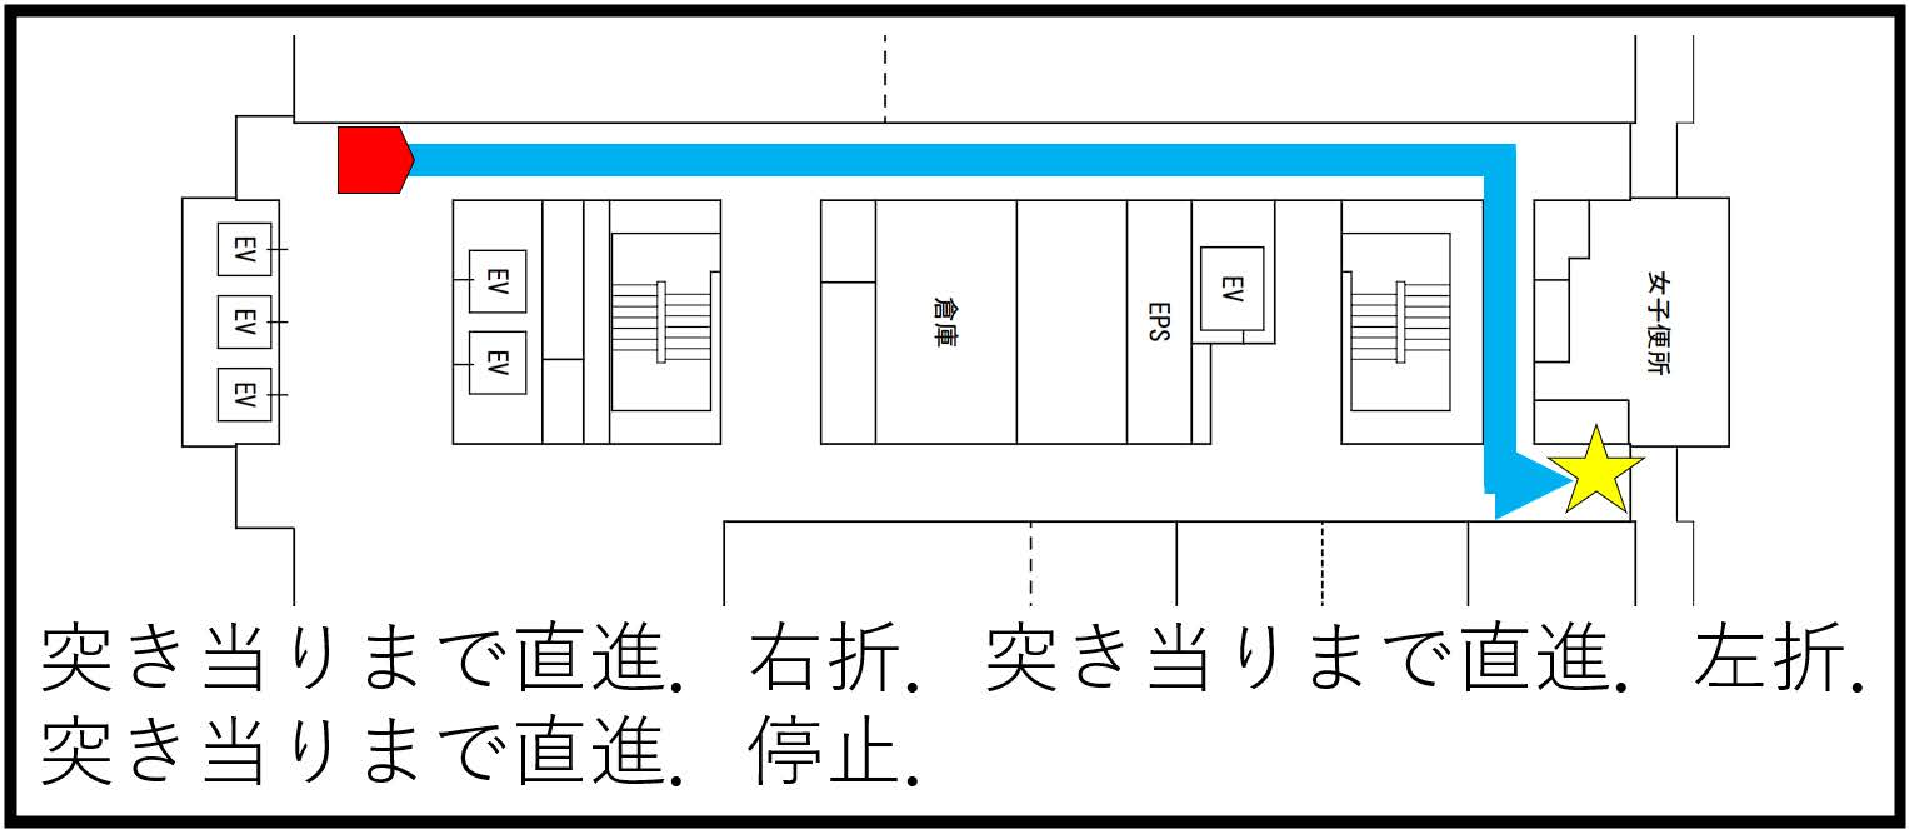
\includegraphics[width=\linewidth]{images/Scenario_07.pdf}
    \caption{Scenario 07}
  \end{subfigure}
  \caption{Scenarios used in the training environment}
  \label{fig:scenario}
\end{figure}

\begin{figure}[p]
  \centering
  \begin{subfigure}[b]{0.32\linewidth}
    \centering
    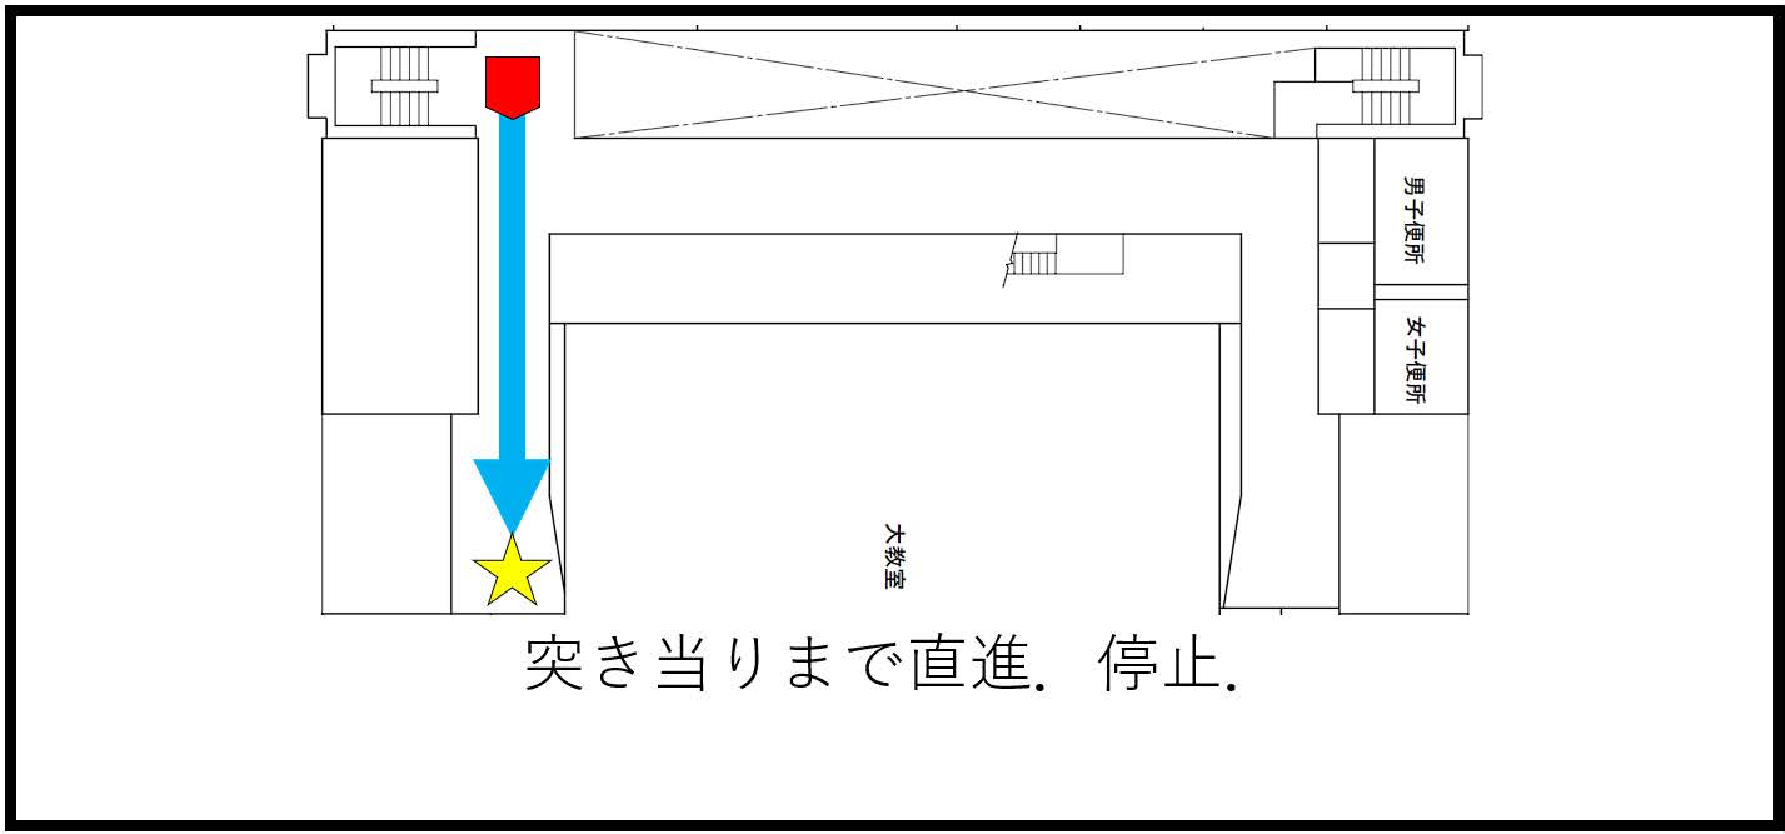
\includegraphics[width=\linewidth]{images/Scenario_16.pdf}
    \caption{Scenario 08}
  \end{subfigure}\hfill
  \begin{subfigure}[b]{0.32\linewidth}
    \centering
    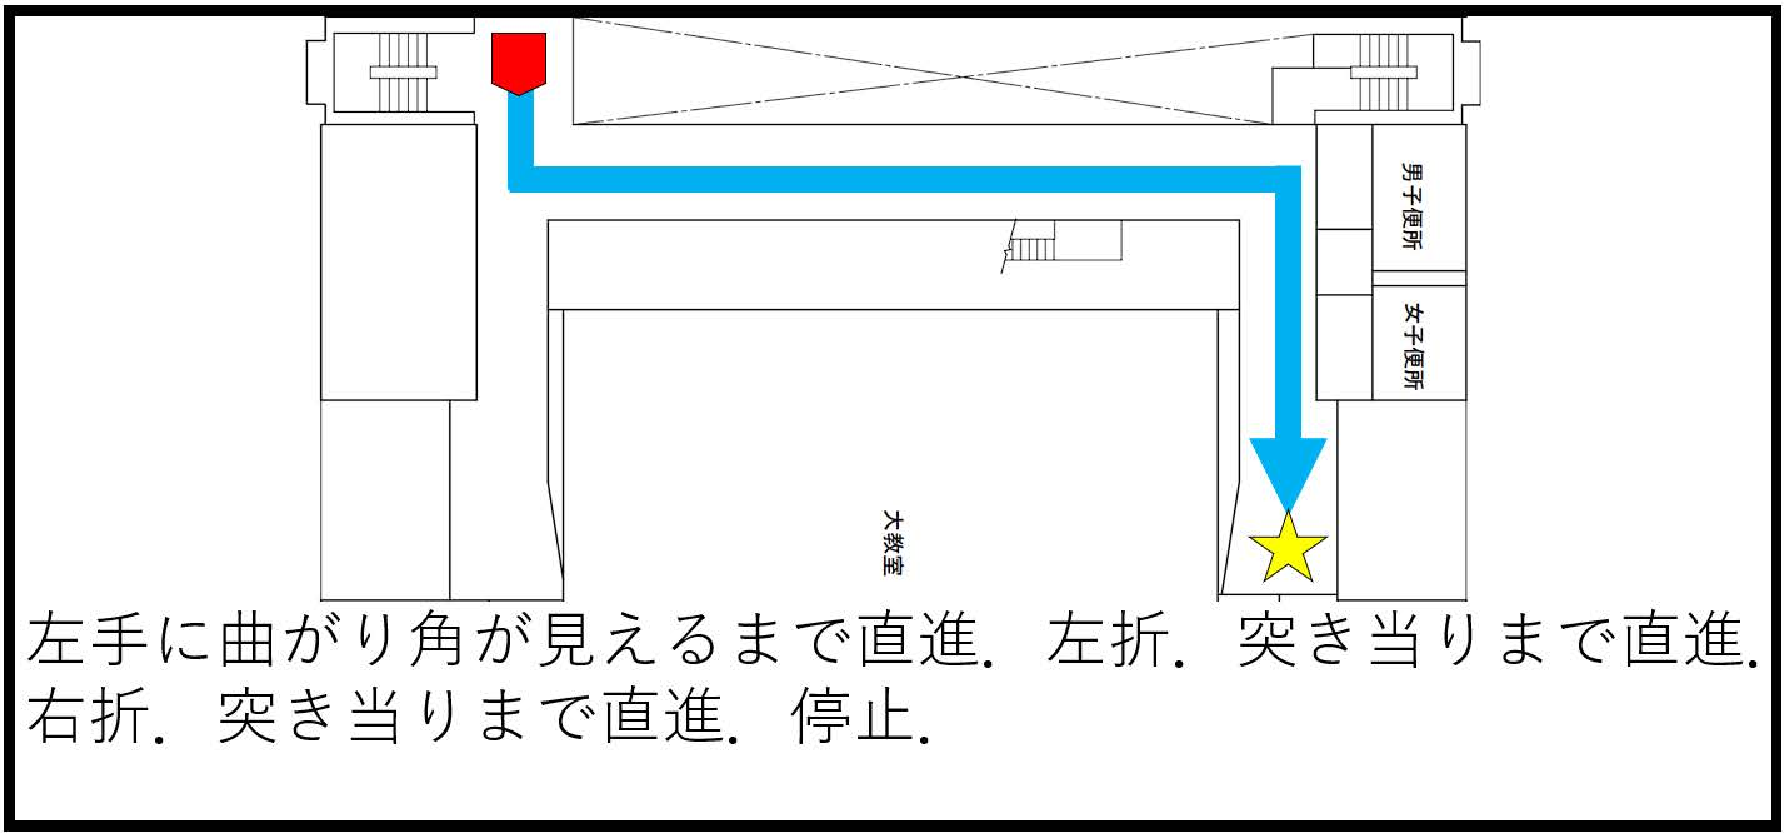
\includegraphics[width=\linewidth]{images/Scenario_17.pdf}
    \caption{Scenario 09}
  \end{subfigure}\hfill
  \begin{subfigure}[b]{0.32\linewidth}
    \centering
    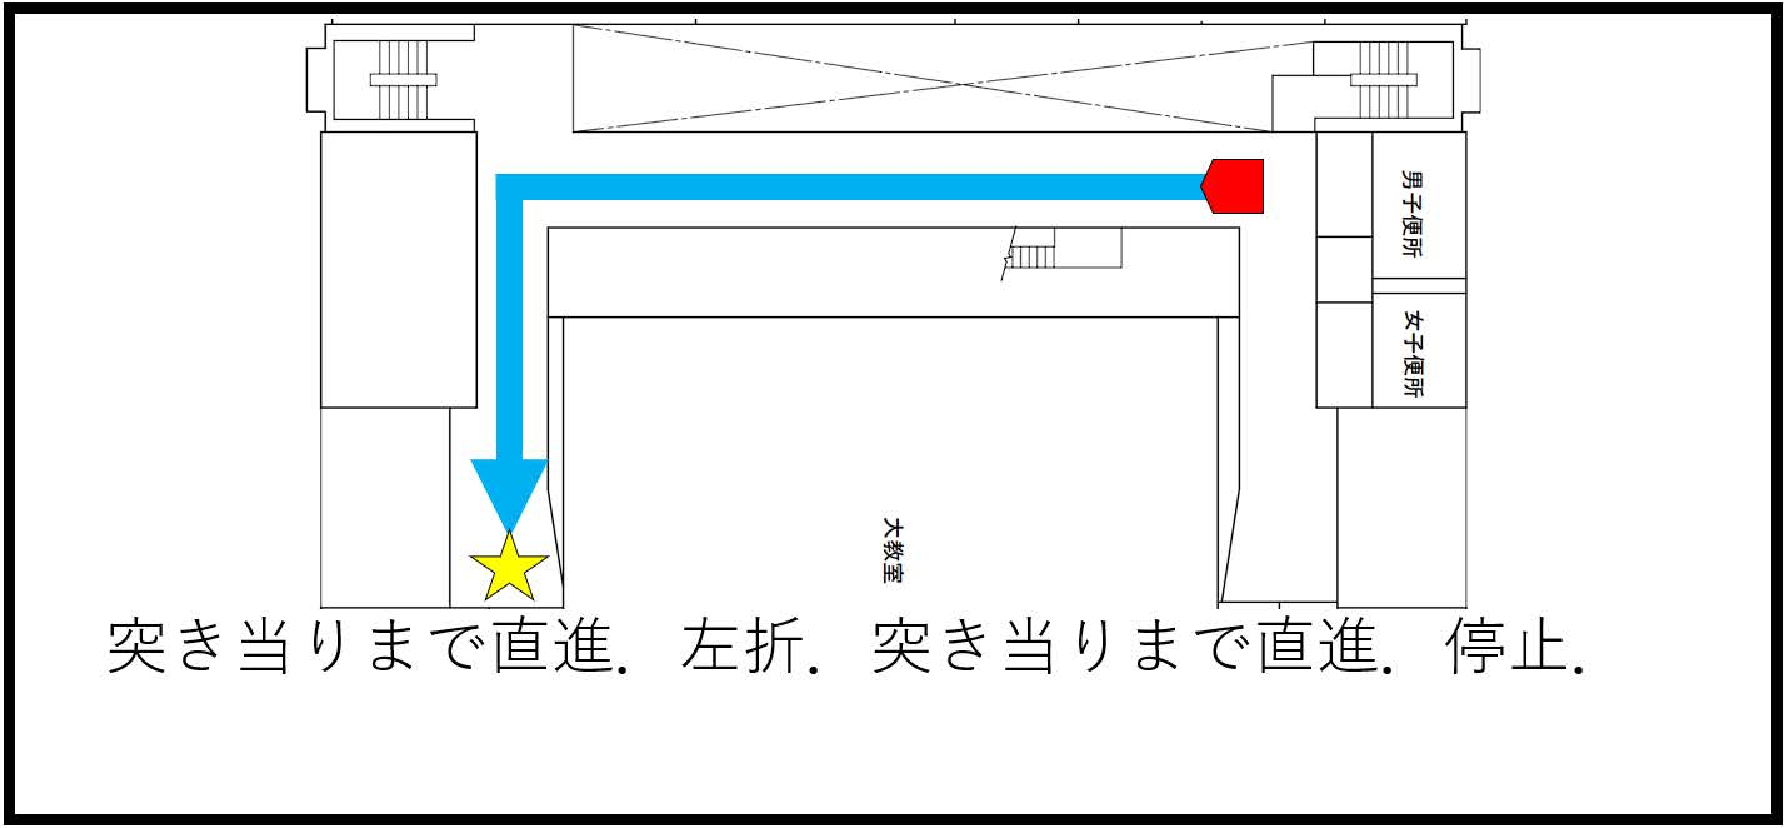
\includegraphics[width=\linewidth]{images/Scenario_27.pdf}
    \caption{Scenario 10}
  \end{subfigure}

  \vspace{0.5\baselineskip}

  \begin{subfigure}[b]{0.32\linewidth}
    \centering
    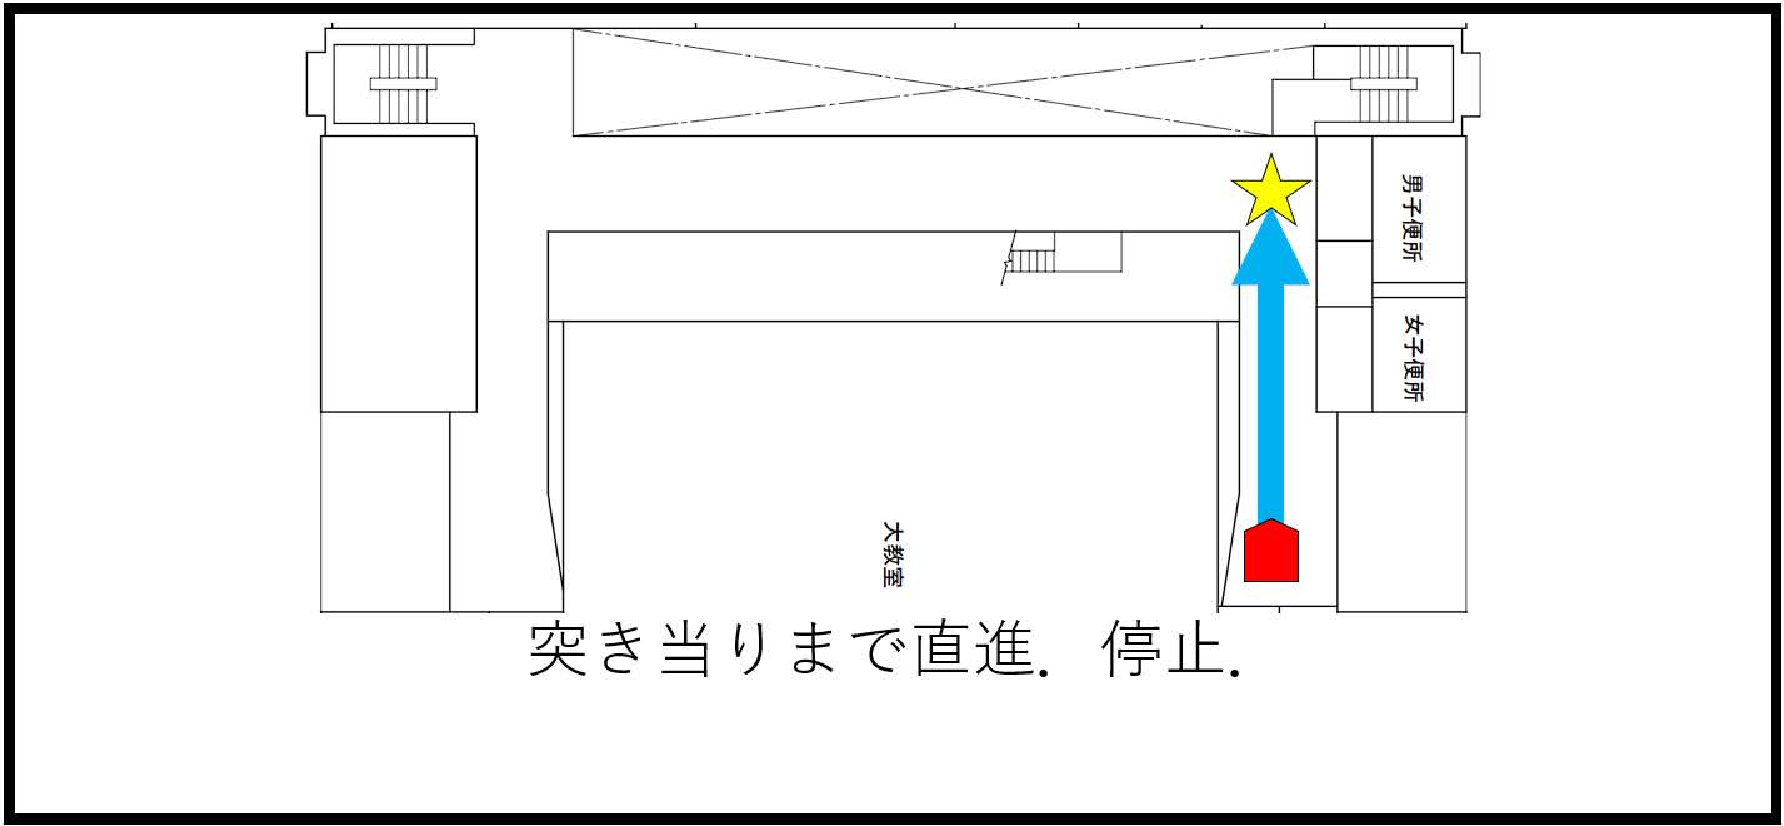
\includegraphics[width=\linewidth]{images/Scenario_31.pdf}
    \caption{Scenario 11}
  \end{subfigure}\hfill
  \begin{subfigure}[b]{0.32\linewidth}
    \centering
    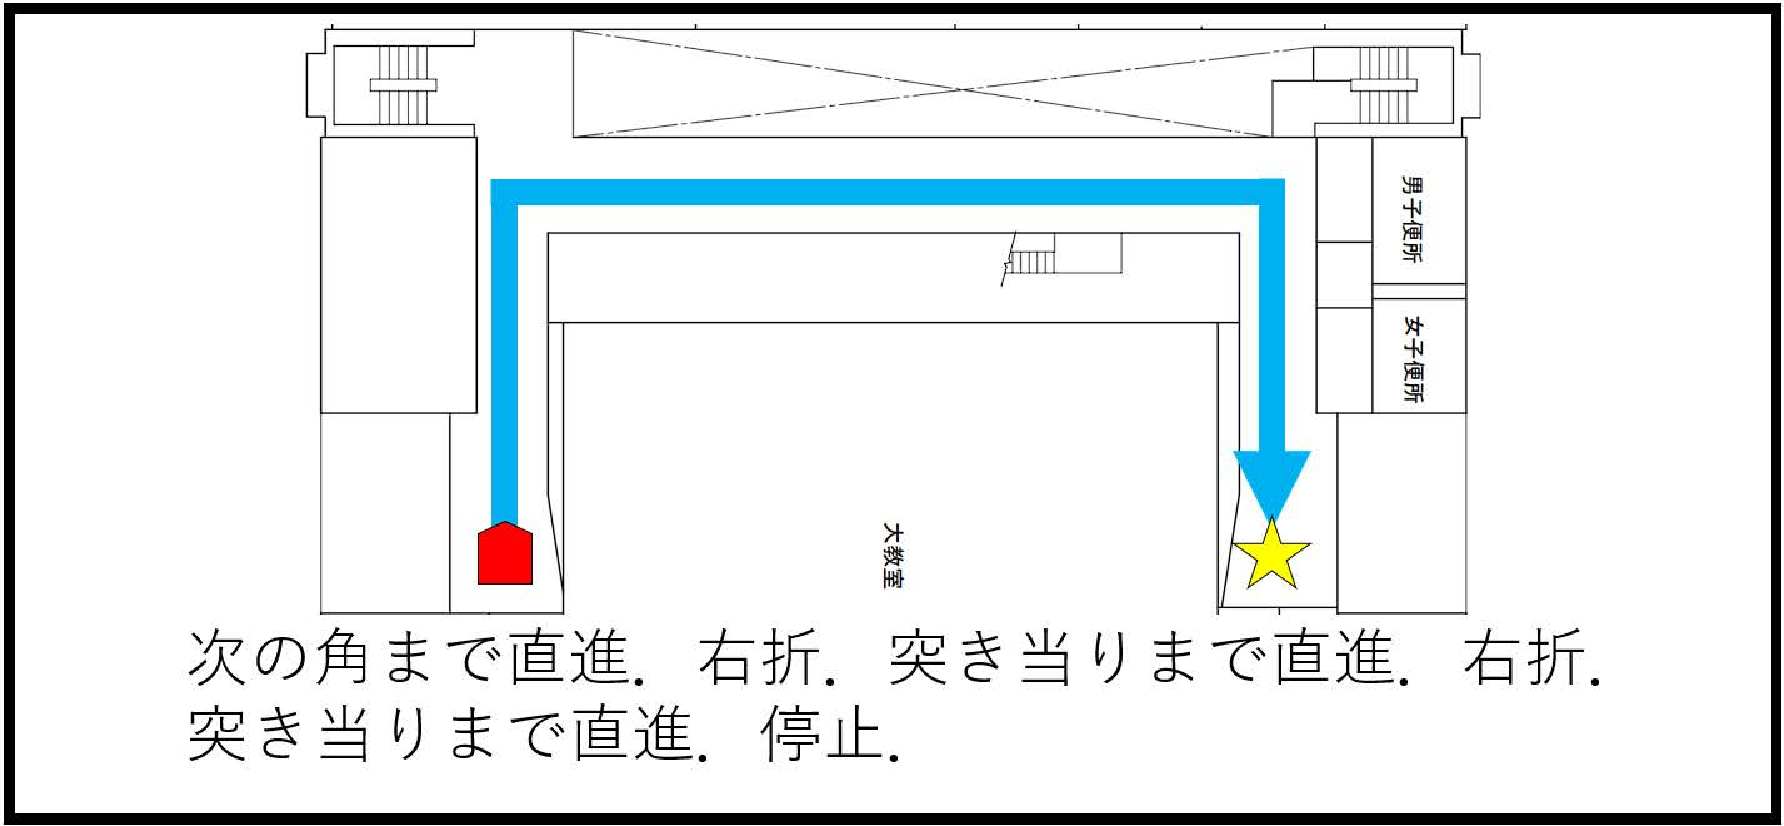
\includegraphics[width=\linewidth]{images/Scenario_36.pdf}
    \caption{Scenario 12}
  \end{subfigure}\hfill
  \begin{subfigure}[b]{0.32\linewidth}
    \centering
    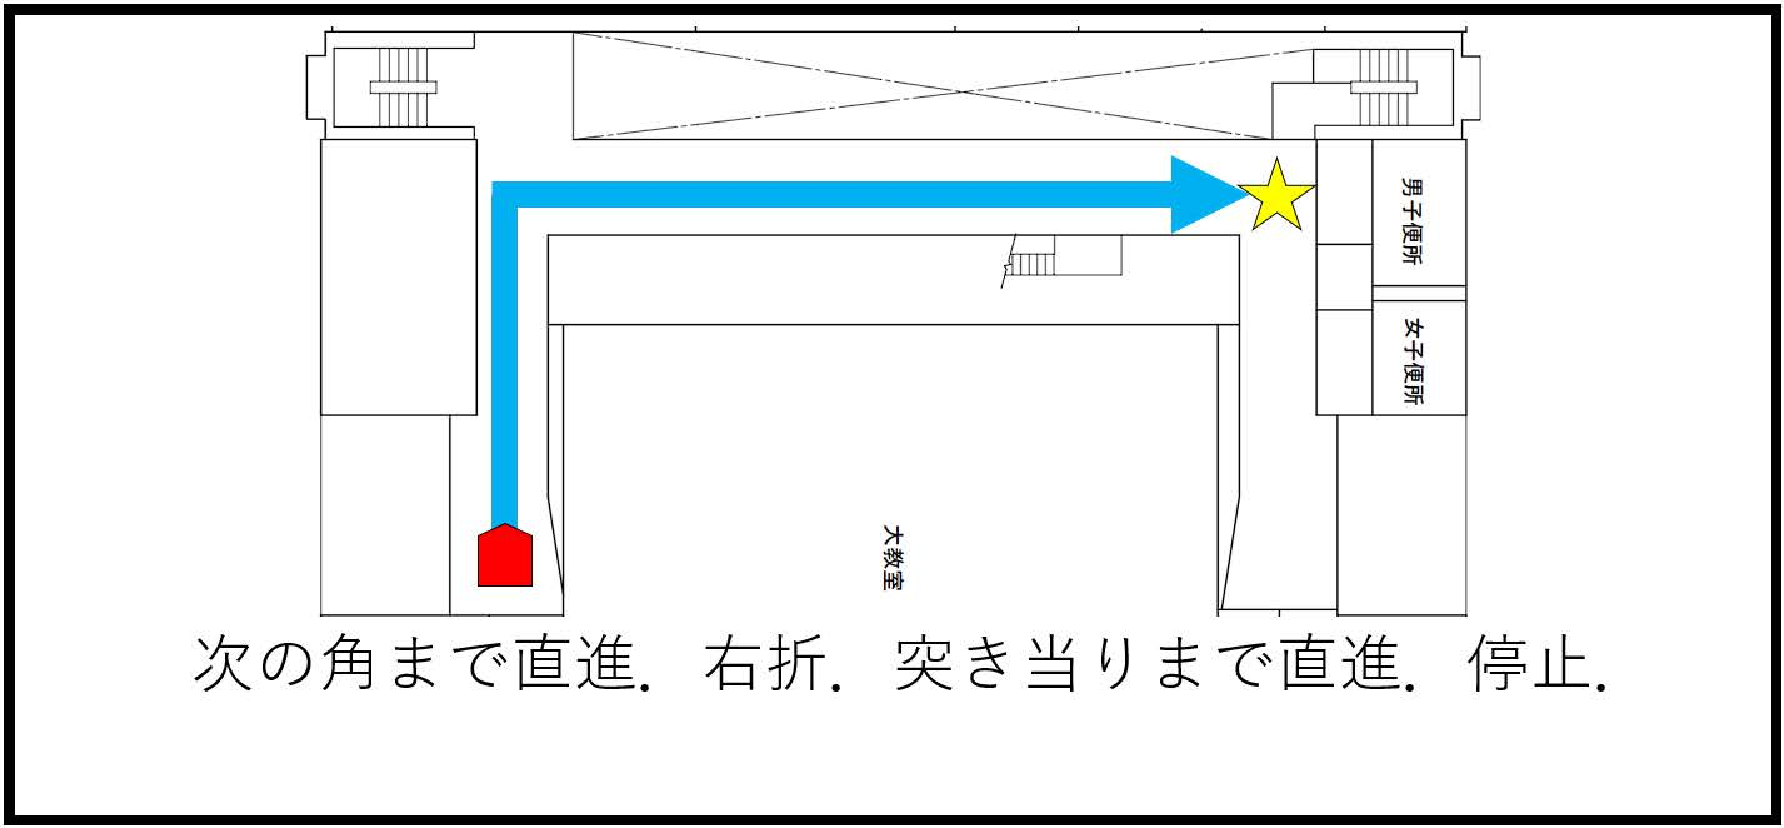
\includegraphics[width=\linewidth]{images/Scenario_37.pdf}
    \caption{Scenario 13}
  \end{subfigure}
  \caption{Scenarios used in the unseen environment}
  \label{fig:scenario_unseen}
\end{figure}

\section{実験結果}
\label{sec:experiment_result}

未学習環境である低層棟でのシナリオ09の走行の様子を\figref{fig:experiment}に示す．
実験の結果，13例すべてのシナリオにおいて，ロボットは目的地まで到達した．
学習環境である高層棟の7例に加え，学習に用いていない低層棟の6例でも到達した．

シナリオ09は，左手の曲がり角まで直進して左折し，突き当りで右折して，次の突き当りで停止する経路である．
このシナリオでは，「左手に曲がり角が見えるまで」と「突き当りまで」の2種類の条件を，未学習環境の画像から判定する必要がある．
% TODO: シナリオ09の走行で，各条件がどこで成立したかを走行ログから書く．

% TODO: シナリオごとの結果（到達の成否，走行時間，衝突の有無など）を表にする．

% TODO: si-paper ではこの図は差し替え予定とされていた（実環境の写真だが，実験はシミュレータ）．
\begin{figure}[tb]
  \centering
  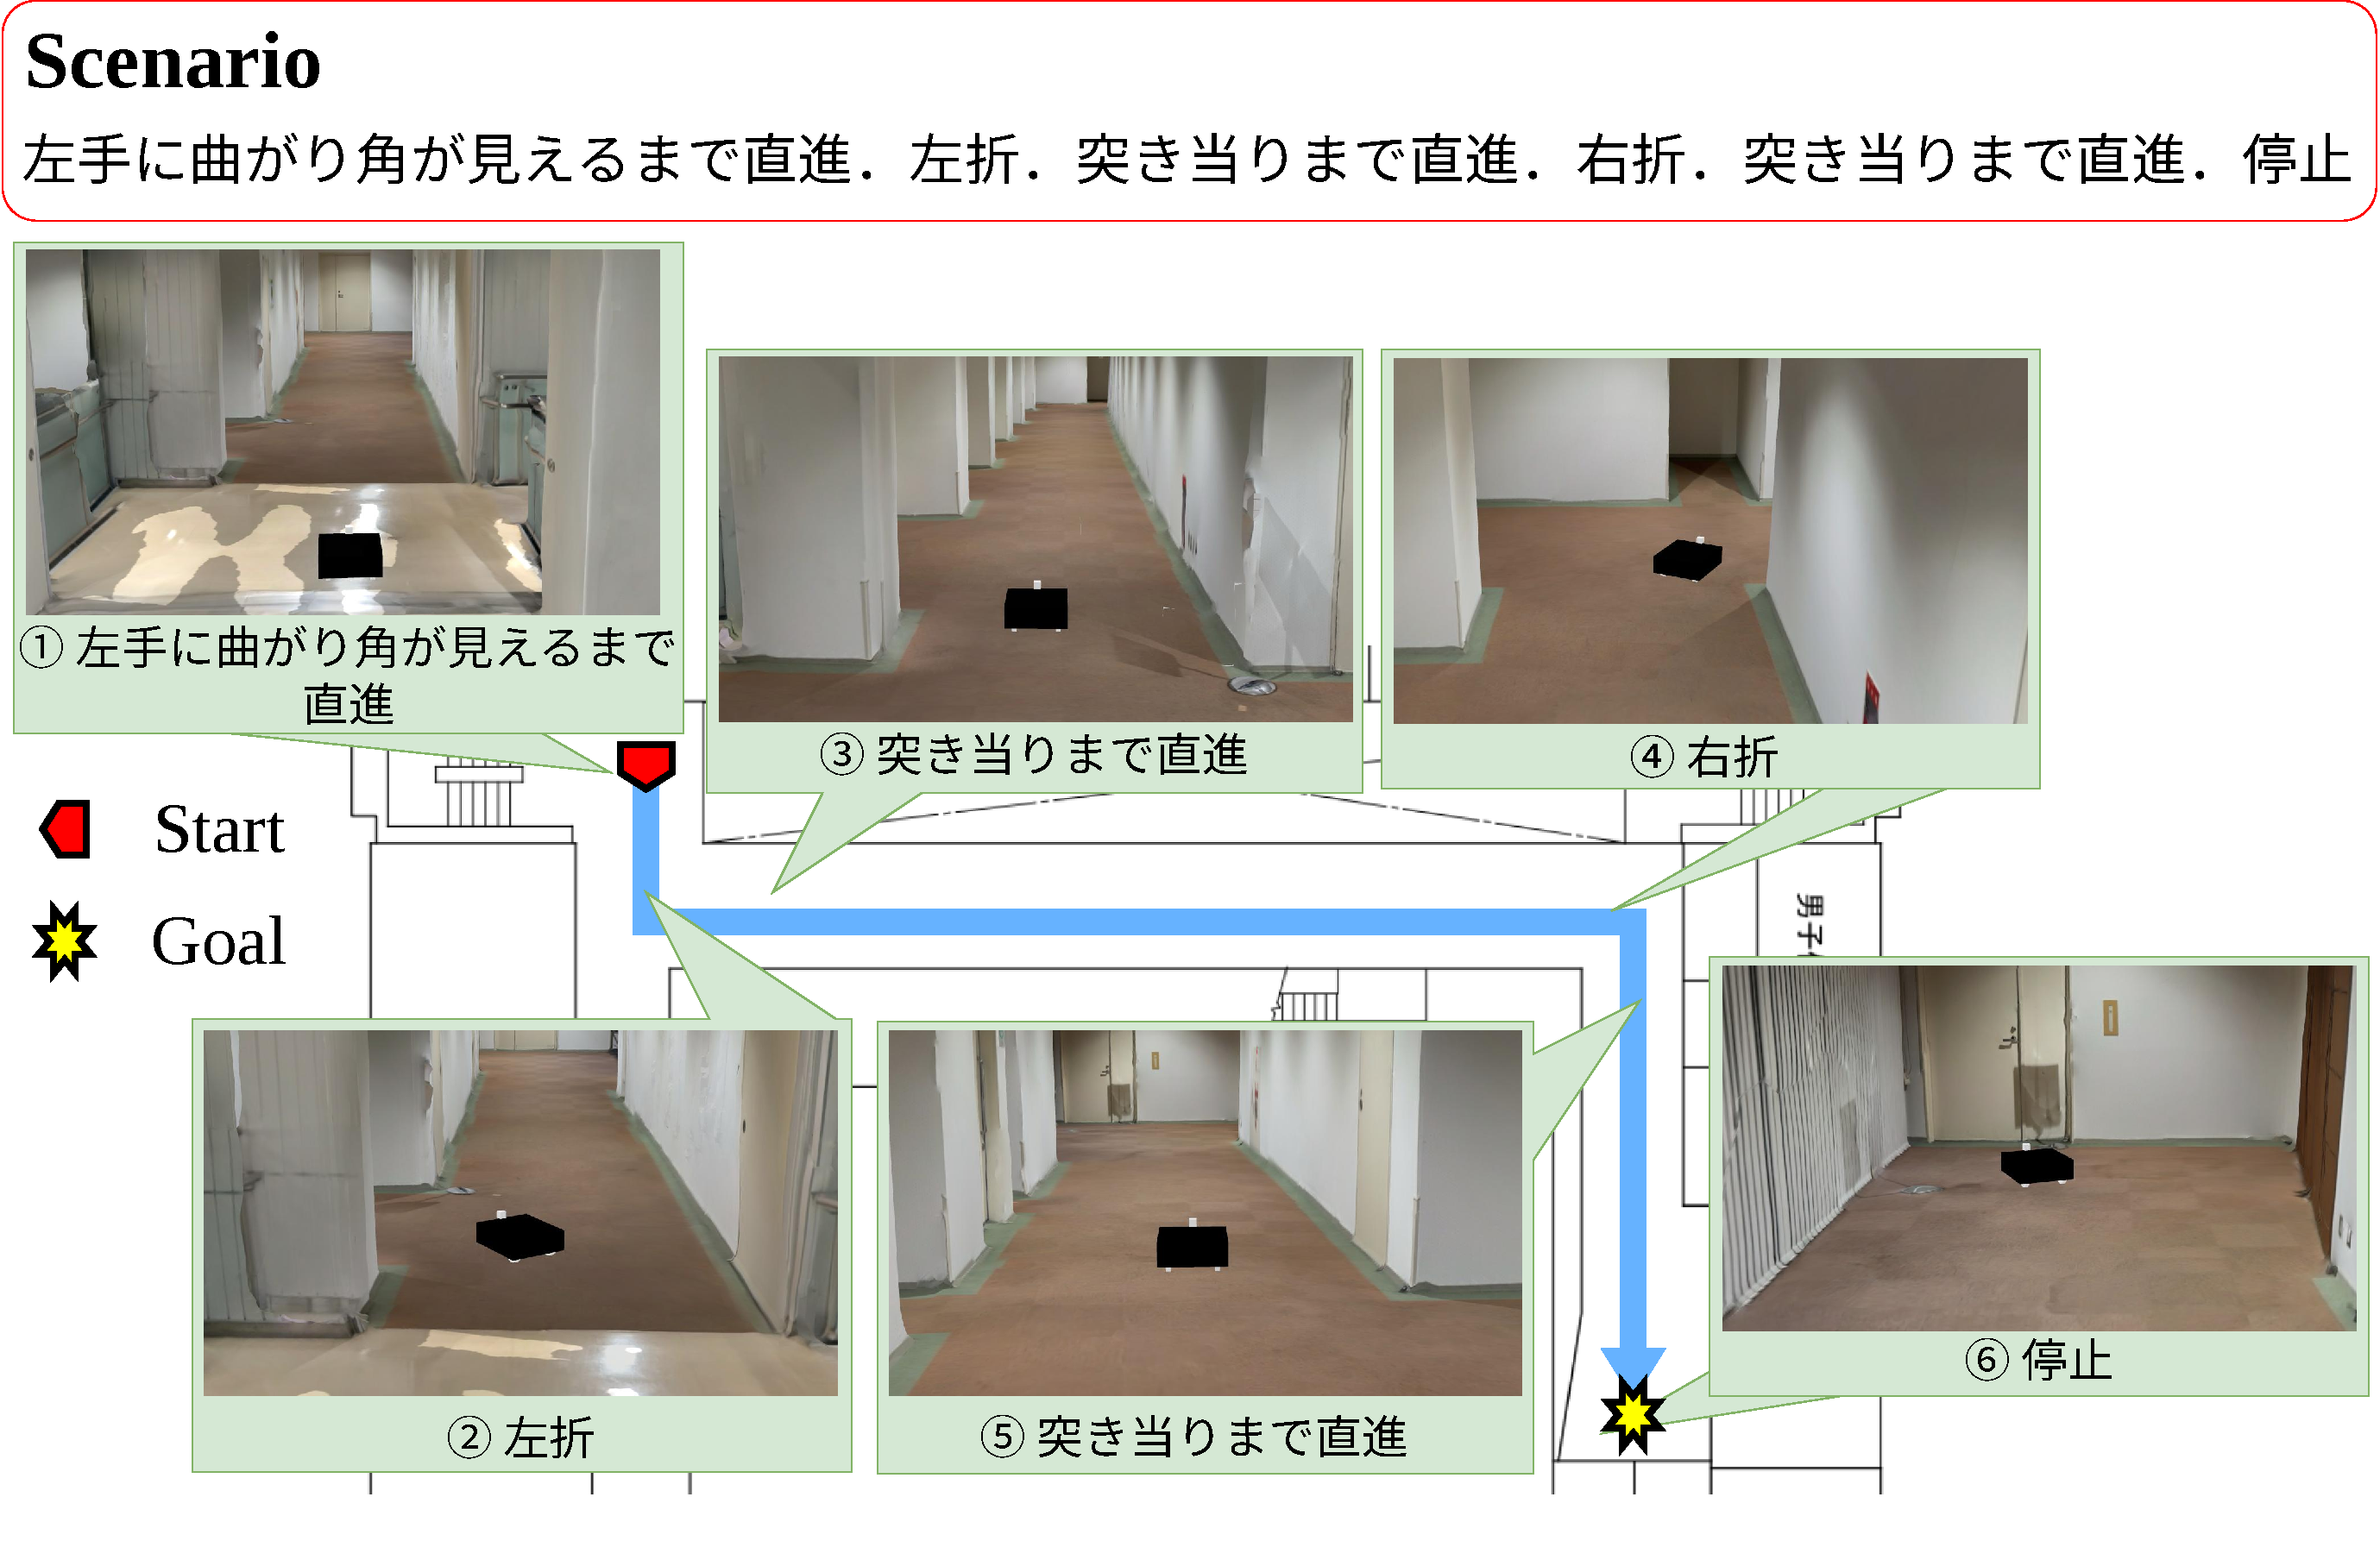
\includegraphics[width=\linewidth]{images/experiment.pdf}
  \caption{Navigation with Scenario 09 in the unseen environment}
  \label{fig:experiment}
\end{figure}

\section{考察}
\label{sec:discussion}

低層棟ではデータ収集やファインチューニングを一切行っていないことから，シミュレータ上の限られた例ではあるが，走行対象の環境でデータ収集や再学習を行わずに，シナリオに従って目的地まで移動できることを確認した．

本実験では，高層棟と低層棟で床や壁の色，エレベーターの有無などの外観が異なる．
それにもかかわらず未学習環境で目的地に到達できた要因として，次の2点が考えられる．
1点目は，\DINOvTwo と\NoMaD の視覚エンコーダを凍結し，事前学習で獲得された表現を保ったことである．
これにより，高層棟の外観に特化した特徴を学習することを避けられたと考えられる．
2点目は，\UniDepth の推定深度から求めた占有格子を通路分類に併用したことである．
占有格子は壁面の位置のみを表し，色や模様の情報を含まないため，外観が異なっても通路の形状を捉えられると考えられる．

一方で，本実験はシミュレータ上の13例に限られる．
また，上記の要因はそれぞれの構成要素を除いた比較を行っていないため，効果を定量的に示したものではない．
実環境では照明の変化や人の往来など，シミュレータにない要因があるため，実環境での評価が必要である．

% TODO: 基盤モデルを凍結した効果，BEVを併用した効果，CAREの効果を比較実験で示すか検討する．
%       corridor_classifier/config/experiments/ に比較の記録（BEV_REPRESENTATION_DECISION.md など）があるので，使えるか確認する．

%!TEX root = ../../thesis.tex
\chapter{実ロボットを用いた実験}
\label{chap:real_world}

% TODO: 本章の概要を書く．

\section{実験装置}
\label{sec:real_setup}

% TODO: ロボット，カメラ，計算機を書く．

\section{実験環境}
\label{sec:real_env}

% TODO: 建物とコース，学習データを収集した環境との関係（未学習環境であること）を書く．

\section{実験方法}
\label{sec:real_method}

% TODO: シナリオ，試行回数，成功の判定基準，記録項目を書く．

\section{実験結果}
\label{sec:real_result}

% TODO: シナリオごとの結果の表と，走行の様子の図．

\section{考察}
\label{sec:real_discussion}

% TODO: 実環境で到達できた要因，残った失敗とその原因，シミュレータとの結果の違いを書く．

%!TEX root = ../../thesis.tex
\chapter{おわりに}
\label{chap:conclusion}

本論文では，目標方向の決定をシナリオが担い，各区間の走行を基盤モデルが担うシステムにより，走行対象の環境での事前走行や再学習，自己位置推定を必要とせずに，シナリオに従って目的地まで移動できるかを検証した．
シミュレータでの検証により，高層棟のデータのみでファインチューニングしたシステムが，学習環境の7例に加え，データを収集していない低層棟の6例においても，シナリオに従って目的地まで到達することを確認した．

本研究では，通路分類モジュールに\DINOvTwo と\UniDepth を，経路追従モジュールに\NoMaD を用いた．
いずれも特徴抽出器を凍結し，通路分類では3方向の有無を推定する部分を，経路追従では目標方向の埋め込みと拡散モデルを学習した．
これにより，用いるモデルのパラメータ数を合計約7500万に抑え，単眼RGBカメラのみで動作するシステムを構成した．

今後の課題を以下に示す．
\begin{itemize}
  \item ロボットに搭載した計算機を用いて，実環境で評価する．
  \item 基盤モデルの凍結や占有格子の併用など，各構成要素の効果を比較実験により定量的に示す．
  \item シナリオの数と試行回数を増やし，到達率や失敗の要因を評価する．
\end{itemize}

% TODO: 今後の課題を書き足す．

% 章を増やすときは chapters/ にディレクトリを作り，ここに追加する

%% Back Matter
\backmatter
\include{backmatter/main}

\end{document}
